\chapter{Background}

\section{Thermodynamic Basics \cite{Floerchinger_2016}}

Take the variation of entropy $S=S(E,N,V)$ in the microcanonical ensemble
\begin{equation}
    \dt S=\frac{1}{T}\dt E-\frac{\mu}{T}\dt N+\frac{p}{T}\dt V
    \label{eq:Thermo_EntropyMicroCan_Differential}
\end{equation}
as a definition of temperature, chemical potential and pressure
\begin{equation}
    \frac{1}{T}=\frac{\partial S}{\partial E}\Big\vert_{N,V}\,,\qquad\mu=-T\frac{\partial S}{\partial N}\Big\vert_{E,V}\,,\qquad p=T\frac{\partial S}{\partial V}\Big\vert_{E,N}
\end{equation}
One also uses inverse temperature $\beta=\frac{1}{T}$ and thermal potential $\alpha=\frac{\mu}{T}$. For homogeneous fluids it is sensible to define densities for energy, particle number and entropy via $E=\epsilon V$, $N=nV$ and $S=sV$. Plugging into the differential \eqref{eq:Thermo_EntropyMicroCan_Differential} gives the \textbf{Gibbs-Duhem relation}
\begin{equation}
    \epsilon+p=Ts+\mu n
    \label{eq:Thermo_GibbsDuhem}
\end{equation}
and
\begin{equation}
    \dt s=\frac{1}{T}\dt\epsilon-\frac{\mu}{T}\dt n
    \label{eq:Thermo_EntropyDensity_Differential}
\end{equation}
(In \cite{Rischke_2022} \eqref{eq:Thermo_GibbsDuhem} multiplied with $V$ is called \textbf{Euler relation}.) Taking the differential of \eqref{eq:Thermo_GibbsDuhem} and using \eqref{eq:Thermo_EntropyDensity_Differential} gives the \textbf{differential Gibbs-Duhem relation}
\begin{equation}
    \dt p=s\dt T+n\dt\mu
    \label{eq:Thermo_DifferentialGibbsDuhem}
\end{equation}

\paragraph*{Legendre Transformations}\mbox{}\\

The function $s(\epsilon,n)$ can be inverted to state a function $\epsilon(s,n)$ that follows
\begin{equation}
    \dt\epsilon=T\dt s+\mu\dt n
\end{equation}
Performing the Legendre transform of $\epsilon(s,n)$ w.r.t. $s$ gives the free energy density
\begin{subequations}
    \begin{align}
        f=f(T,n) & =\epsilon-Ts      \\
        \dt f    & =-s\dt T+\mu\dt n
    \end{align}
\end{subequations}
and another Legendre transform w.r.t. $n$ leads to
\begin{subequations}
    \begin{align}
        -p=-p(T,\mu) & =f-\mu n         \\
        -\dt p       & =-s\dt T-n\dt\mu
    \end{align}
\end{subequations}
hence the pressure is just another thermodynamic potential.

\section{Fluid Dynamic Approach}

The theory of fluid dynamics aims to describe a system of many interacting particles as a fluid, with its state specified by a few spacetime dependent variables, such as temperature $T(x)$ and chemical potential $\mu(x)$, and an equation of state. Dynamics are generated by equations of motion involving the energy-momentum tensor $T^{\mu\nu}(x)$.
\begin{equation}
    \begin{split}
        T^{00}\dots\,&\text{local energy density}\\
        T^{i0}\dots\,&\text{local momentum density}\\
        T^{\mu j}\dots\,&\text{flux of }\mu\text{-component in direction }j
    \end{split}
\end{equation}
\todo{Why is $T^{\mu\nu}$ symmetric?}\todo{Why does this coincide with the definition $T^{\mu\nu}$ from a Lagrangian?}
In a local rest frame the energy-momentum tensor should have the form of static equilibrium. There should be further no flow of particle number or entropy, specifying the form of the particle and entropy current $N^\mu$ and $S^\mu$. In a rest frame one finds
\begin{subequations}
    \begin{align}
        T^{\mu\nu}_{RF} & =
        \begin{pmatrix}
            \epsilon & 0 & 0 & 0 \\
            0        & P & 0 & 0 \\
            0        & 0 & P & 0 \\
            0        & 0 & 0 & P
        \end{pmatrix}
        \label{eq:FluidMechanics_EnMomTens_RestFrame} \\
        N^\mu_{RF}      & =(n,0,0,0)^T                \\
        S^\mu_{RF}      & =(s,0,0,0)^T
    \end{align}
    \label{eq:FluidMechanics_RestFrame_Quantities}
\end{subequations}
with energy density $\epsilon$ and pressure $P$. \todo{Check why kinetic and thermodynamic pressure coincide.}

In a general frame these quantitites are obtained by applying a Lorentz boost to \eqref{eq:FluidMechanics_RestFrame_Quantities} and read \cite{Rischke_2022}
\begin{subequations}
    \begin{align}
        T^{\mu\nu} & =-Pg^{\mu\nu}+(P+\epsilon)u^\mu u^\nu=\epsilon u^\mu u^\nu-\Delta^{\mu\nu}P \\
        N^\mu      & =nu^\mu                                                                     \\
        S^\mu      & =su^\mu
    \end{align}
\end{subequations}
where $u^\mu=(\gamma,\gamma\mathbf{v})$ is the local fluid 4-velocity and $\Delta^{\mu\nu}=g^{\mu\nu}-u^\mu u^\nu$ is the projector orthogonal to $u^\mu$. It fulfills
\begin{equation}
    \Delta^{\mu\nu}=\Delta^{\nu\mu}\,,\qquad u_\mu\Delta^{\mu\nu}=0\,,\qquad\Delta^\mu_\lambda\Delta^{\lambda\nu}=\Delta^{\mu\nu}\,\qquad\Delta^\mu_\mu=3=d-1
    \label{eq:FluidMechanics_ProjProperties}
\end{equation}
Signature is chosen such that $u_\mu u^\mu=1$.
\begin{impt}[Signature Convention]{impt:SignatureConvention}
    \begin{equation*}
        \eta^{\mu\nu}=\text{diag}(+,-,-,-)
    \end{equation*}
\end{impt}

Local energy-momentum conservation and particle number conservation are encoded by the continuity equations
\begin{subequations}
    \begin{align}
        \partial_\mu T^{\mu\nu} & =0 \label{eq:FluidMechanics_EnMomTens_Conservation}  \\
        \partial_\mu N^\mu      & =0 \label{eq:FluidMechanics_PartNumCur_Conservation}
    \end{align}
\end{subequations}
which constitutes 5 scalar equations for 6 unkwon functions: $\epsilon(x), P(x), n(x), \mathbf{v}(x)$. The equation of state $P=P(\epsilon,n)$ closes the system.

\begin{calc}[Symmetry of $T^{\mu\nu}$]{calc:FluidMechanics_EnMomTensSymm_AngulMom}
    The angular momentum tensor is defined as
    \begin{equation}
        J^{\lambda,\mu\nu}=x^\mu T^{\lambda\nu}-x^\nu T^{\lambda\mu}
        \label{eq:FluidMechanics_AngularMomentum_Def}
    \end{equation}
    Angular momentum conservation gives
    \begin{align*}
        0 & =\partial_\lambda J^{\lambda,\mu\nu}                                                                               \\
          & =T^{\mu\nu}-T^{\nu\mu}+\underbrace{x^\mu\partial_\lambda T^{\lambda\nu}-x^\nu\partial_\lambda T^{\lambda\mu}}_{=0} \\
          & =T^{\mu\nu}-T^{\nu\mu}
    \end{align*}
    where conservation of energy-momentum \eqref{eq:FluidMechanics_EnMomTens_Conservation} was used.
\end{calc}

\subsection{Covariant Thermodynamics and Entropy Production}

The goal is to rewrite the thermodynamic equilibrium equations in a covariant form. Introduce
\begin{equation}
    \beta^\mu=\frac{u^\mu}{T}
\end{equation}
and postulate
\begin{subequations}
    \begin{align}
        \dt(P\beta^\mu) & =N^\mu\dt\alpha-T^{\mu\nu}\dt\beta_\nu       \\
        S^\mu           & =P\beta^\mu+T^{\mu\nu}\beta_\nu-\alpha N^\mu
    \end{align}
    which immediately implies
    \begin{equation}
        \dt S^\mu=\beta_\nu\dt T^{\mu\nu}-\alpha\dt N^\mu
        \label{eq:FluidMechanics_DifferentialGibbsDuhem_Covariant}
    \end{equation}
    \label{eq:FluidMechanics_CovariantThermo_Postulates}
\end{subequations}
Upon contraction with $u_\mu$ equations \eqref{eq:FluidMechanics_CovariantThermo_Postulates} yield again \eqref{eq:Thermo_GibbsDuhem}, \eqref{eq:Thermo_EntropyDensity_Differential} and \eqref{eq:Thermo_DifferentialGibbsDuhem}.

Equation \eqref{eq:FluidMechanics_DifferentialGibbsDuhem_Covariant} furher implies \todo{Why exactly can we replace the $\dt$ with a $\partial_\mu$?}
\begin{equation}
    \partial_\mu S^\mu=\beta_\nu\partial_\mu T^{\mu\nu}-\alpha\partial_\mu N^\mu
\end{equation}
Assuming conservation of energy-momentum and particle number leads to conservation of entropy,
\begin{equation}
    \partial_\mu S^\mu=0
\end{equation}
which holds in thermal equilibrium.

It is also possible to postulate conservation of energy-momentum and particle number and entropy in thermal equilibrium and infer the differential form \eqref{eq:FluidMechanics_DifferentialGibbsDuhem_Covariant}.

% \subsection{Dissipative Effects}

% Real fluids are not in exact local thermodynamic equilibrium. Instead, irreversible processes dissipate energy and increase entropy. to lowest order this is modelled by adding dissipative currents to $n^\mu$ and $\tau^{\mu\nu}$ to the previously discussed ideal currents.
% \begin{subequations}
%     \begin{align}
%         N^\mu      & =N^\mu_{(0)}+n^\mu              =n_0u^\mu+n^\mu                                         \\
%         T^{\mu\nu} & =T_{(0)}^{\mu\nu}+\tau^{\mu\nu} =\epsilon_0u^\mu u^\nu-\Delta^{\mu\nu}P_0+\tau^{\mu\nu}
%     \end{align}
% \end{subequations}
% The ideal currents with index $\#_{(0)}$ are now ill defined. One imposes the \textbf{Landau matching conditions}
% \begin{subequations}
%     \begin{align}
%         \epsilon_0 & \equiv\epsilon=u_\mu u_\nu T^{\mu\nu} \\
%         n_0        & \equiv n=u_\mu N^\mu
%     \end{align}
% \end{subequations}
% implying the constraints
% \begin{subequations}
%     \begin{align}
%         u_\mu u_\nu\tau^{\mu\nu} & =0                                                     \\
%         u_\mu n^\mu              & =0 \quad \iff \quad \Delta^\mu_\lambda n^\lambda=n^\mu
%     \end{align}
% \end{subequations}

% Defining entropy density $s_0\equiv s_0(\epsilon,n)$ as if the system was in equilibrium with state variables $(\epsilon,n)$ other thermodynamic variables are derived from $s_0$ as before. Whereas energy and particle density are well-defined, other quantitites ($s_0,P_0,T_0,\mu_0,\dots$) are defined only w.r.t. a fictitious equilibrium state which is not directly restricted by the laws of thermodynamics.

\subsection{Derivative Expansion of hydrodynamics \cite{Kovtun_2012}}

Given some vector $u^\mu(x)$, any spacetime tensor can be decomposed as
\begin{subequations}
    \begin{align}
        T^{\mu\nu} & =\mathcal{E} u^\mu u^\nu+\mathcal{P}\Delta^{\mu\nu}+(q^\mu u^\nu+q^\nu u^\mu)+t^{\mu\nu}\label{eq:FluidMechanics_EnMomTens_Decomposition} \\
        J^\mu      & =\mathcal{N}u^\mu+j^\mu\label{eq:FluidMechanics_Vector_Decomposition}
    \end{align}
    \label{eq:FluidMechanics_Tensor_Decomposition}
\end{subequations}
with the coefficients given by
\begin{subequations}
    \begin{gather}
        \mathcal{E}=u_\mu u_\nu T^{\mu\nu}\,,\quad \mathcal{P}=\frac{1}{d}\Delta_{\mu\nu}T^{\mu\nu}\,,\quad \mathcal{N}=u_\mu J^\mu\\
        q_\mu=\Delta_{\mu\alpha}u_\beta T^{\alpha\beta}\,,\quad j_\mu=\Delta_{\mu\nu}J^\nu\\
        t_{\mu\nu}=\frac{1}{2}\Big(\Delta_{\mu\alpha}\Delta_{\nu\beta}+\Delta_{\nu\alpha}\Delta_{\mu\beta}-\frac{2}{d-1}\Delta_{\mu\nu}\Delta_{\alpha\beta}\Big)T^{\alpha\beta}
    \end{gather}
    \label{eq:FluidMechanics_Tensor_DecompositionCoefficients}
\end{subequations}

\begin{calc}[Decomposition of Rank-1 and Rank-2 Spacetime Tensors]{calc:FluidMechanics_TensorDecomposition}
    Use $u_\mu u^\mu=1$ as well as $\Delta^{\mu\nu}+u^\mu u^\nu=g^{\mu\nu}$ (or $\Delta^\mu_\nu+u^\mu u_\nu=\delta^\mu_\nu$) and the projector properties \eqref{eq:FluidMechanics_ProjProperties}.


    \begin{align*}
        J^\mu      & =\delta^\mu_\nu J^\nu                                                                                                                                                                                                                                                       \\
                   & =(\Delta^\mu_\nu+u^\mu u_\nu)J^\nu                                                                                                                                                                                                                                          \\
                   & =j^\mu +\mathcal{N}u^\mu                                                                                                                                                                                                                                                    \\
        T^{\mu\nu} & =\delta^\mu_\alpha\delta^\nu_\beta T^{\alpha\beta}                                                                                                                                                                                                                          \\
                   & =(\Delta^\mu_\alpha+u^\mu u_\alpha)(\Delta^\nu_\beta+u^\nu u_\beta)T^{\alpha\beta}                                                                                                                                                                                          \\
                   & =(\Delta^\mu_\alpha\Delta^\nu_\beta+\Delta^\nu_\beta u^\mu u_\alpha+\Delta^\mu_\alpha u^\nu u_\beta + u^\mu  u^\nu u_\alpha u_\beta)T^{\alpha\beta}                                                                                                                         \\
                   & =(\Delta^\mu_\alpha\Delta^\nu_\beta-\frac{1}{d-1}\Delta^{\mu\nu}\Delta_{\alpha\beta}+\frac{1}{d-1}\Delta^{\mu\nu}\Delta_{\alpha\beta}+\Delta^\nu_\beta u^\mu u_\alpha+\Delta^\mu_\alpha u^\nu u_\beta + u^\mu  u^\nu u_\alpha u_\beta)T^{\alpha\beta}                       \\
        \intertext{\dots using symmetry of $T^{\alpha\beta}$\dots}
                   & =\frac{1}{2}\Big(\Delta^\mu_\alpha\Delta^\nu_\beta+\Delta^\nu_\alpha\Delta^\mu_\beta-\frac{2}{d-1}\Delta^{\mu\nu}\Delta_{\alpha\beta}\Big)T^{\alpha\beta}+\frac{1}{d-1}\Delta^{\mu\nu}\Delta_{\alpha\beta}T^{\alpha\beta}+(q^\nu u^\mu+q^\mu u^\nu)+\mathcal{E} u^\mu u^\nu \\
                   & =t^{\mu\nu}+\mathcal{P}\Delta^{\mu\nu}+(q^\nu u^\mu+q^\mu u^\nu)+\mathcal{E} u^\mu u^\nu
    \end{align*}

    Show $t^{\mu\nu}$ is constructed to be transverse $t^{\mu\nu}u_\nu=0$ and traceless:
    \begin{equation*}
        \Delta^{\mu\nu}t_{\mu\nu} =\frac{1}{2}\Big(\underbrace{\Delta^\nu_\alpha\Delta_{\nu\beta}+\Delta_{\nu\alpha}\Delta^\nu_\beta}_{=2\Delta_{\alpha\beta}}-\frac{2}{d-1}(d-1)\Delta_{\alpha\beta}\Big)T^{\alpha\beta}=0
    \end{equation*}
\end{calc}
The object
\begin{equation}
    \Delta^{\mu\nu}_{\alpha\beta}=\frac{1}{2}\Big(\Delta_{\mu\alpha}\Delta_{\nu\beta}+\Delta_{\nu\alpha}\Delta_{\mu\beta}-\frac{2}{d-1}\Delta_{\mu\nu}\Delta_{\alpha\beta}\Big)=\frac{1}{2}\Big(\Delta_{\mu\alpha}\Delta_{\nu\beta}+\Delta_{\nu\alpha}\Delta_{\mu\beta}-\frac{2}{\Delta^\lambda_\lambda}\Delta_{\mu\nu}\Delta_{\alpha\beta}\Big)
\end{equation}
has some properties \todo{Maybe list the properties here.}

\subsubsection{$0$th Order Hydrodynamics}

Ideal hydrodynamics corresponds to the $0$th order in a derivative expansion of the (scalar) hydrodynamic variables \todo{There only scalar hydrodynamic variables, except $u^\mu$, right?}. The tensors $q^\mu$, $t^{\mu\nu}$ can only contain derivatives and hence drop out to lowest order. The $0$th order coefficients are identified with the energy density, pressure and particle density of an ideal fluid in thermodynamic equilbrium in a rest frame and promoted to slowly varying fields. One finds
\begin{subequations}
    \begin{align}
        T^{\mu\nu}_{(0)} & =\epsilon u^\mu u^\nu-p\Delta^{\mu\nu} =(\epsilon+p)u^\mu u^\nu-pg^{\mu\nu} \\
        N^\mu_{(0)}      & =nu^\mu
    \end{align}
\end{subequations}
Given an equation of state $p(T,\mu)$ entropy and particle number density is found using \eqref{eq:Thermo_DifferentialGibbsDuhem} and subsequently energy density via \eqref{eq:Thermo_GibbsDuhem}. Enthalpy density is given by
\begin{equation}
    w=\epsilon+p
\end{equation}
The (longitudinal components of) energy-momentum conservation and particle number conservation read
\begin{subequations}
    \begin{align}
        0 & =u_\nu\partial_\mu T^{\mu\nu}=u^\mu\partial_\mu\epsilon+\epsilon\partial_\mu u^\mu+p\Delta^{\mu\nu}\partial_\mu u_\nu=\partial_\mu(\epsilon u^\mu)+p\partial_\mu u^\mu=\partial_\mu(wu^\mu)-u^\mu\partial_\mu p \\
        0 & = \partial_\mu (nu^\mu)
    \end{align}
    \label{eq:FluidMechanics_0thOrderConservationLaws}
\end{subequations}
where $0=u^\nu\partial_\mu u_\nu$ or equivalently $\partial_\mu u_\lambda=\Delta^\nu_\lambda\partial_\mu u_\nu$ as well as $\Delta^{\mu\nu}u_\nu=0$ which implies $\Delta^{\mu\nu}\partial_\lambda u_\nu=-u_\nu\partial_\lambda\Delta^{\mu\nu}$ was used. Using $w=sT+\mu n$ one can compute
\begin{align*}
    \partial_\mu(w u^\mu) & =T\partial_\mu(su^\mu)+su^\mu\partial_\mu T+\mu\partial_\mu (nu^\mu)+nu^\mu\partial_\mu\mu                                                                \\
                          & =T\partial_\mu(su^\mu)+\mu\partial_\mu (nu^\mu)+u^\mu\Big(\frac{\partial p}{\partial T}\partial_\mu T+\frac{\partial p}{\partial \mu}\partial_\mu\mu\Big) \\
                          & =T\partial_\mu(su^\mu)+\mu\cdot 0+u^\mu\partial_\mu p                                                                                                     \\
    \overset{!}           & {=}u^\mu\partial_\mu p\quad\implies\quad\partial_\mu(su^\mu)=0
\end{align*}
to show conservation of the entropy current.

\subsubsection{$1$st Order Hydrodynamics}

Including first derivatives the coefficients \eqref{eq:FluidMechanics_Tensor_DecompositionCoefficients} take the form
\begin{subequations}
    \begin{align}
        \mathcal{E}(x) & =\epsilon(x)+f_{\mathcal{E}}(\partial T,\partial\mu,\partial u^\mu) \\
        \mathcal{P}(x) & =-p(x)+f_{\mathcal{P}}(\partial T,\partial\mu,\partial u^\mu)       \\
        \mathcal{N}(x) & =n(x)+f_{\mathcal{N}}(\partial T,\partial\mu,\partial u^\mu)
    \end{align}
\end{subequations}

Understanding $T,\mu,u^\mu$ as auxiliary fields in the parametrization of $T^{\mu\nu}$, changing the parametrization \todo[I imagine it like this: In my system I choose a spacetime point $x_0$ and take the corresponding $T(x_0), p(x_0), u^\mu(x_0)$. If $\mu,T,u^\mu$ where constant, boosting into the local frame with $u^\mu(x_0)$ enables me to read off $\epsilon_0,p_0,n_0$.]{Why exactly are the coefficients of $T^{\mu\nu}$ not exactly the energy density and pressure, but only up to derivatives of hydro variables? Does the expansion or the precise form of $f_{\mathcal{E}}\dots$ depend on the spacetime point $x$?}
\begin{subequations}
    \begin{align}
        T(x)     & \to T^\prime(x)=T(x)+\delta T(x)              \\
        \mu(x)   & \to \mu^\prime(x)=\mu(x)+\delta\mu(x)         \\
        u^\mu(x) & \to u^{\mu\prime}(x)=u^\mu(x)+\delta u^\mu(x)
    \end{align}
\end{subequations}
where $\delta(u^\mu u_\mu)=0$ implies $u_\mu\delta u^\mu=0$ and demanding invariance of $T^{\mu\nu}$ and $J^\mu$ changes the coefficients \eqref{eq:FluidMechanics_Tensor_DecompositionCoefficients} to first order by\todo{Do this explicitly, especially for $t^{\mu\nu}$ it is hard to see.}
\begin{subequations}
    \begin{gather}
        \delta\mathcal{E}=0\,,\quad\delta\mathcal{P}=0\,,\quad\delta\mathcal{N}=0\label{eq:FluidMechanics_FrameVariation_ScalarTensCoeffs}\\
        \delta q^\mu=-(\mathcal{E}-\mathcal{P})\delta u^\mu\,,\quad\delta j^\mu=-\mathcal{N}\delta u^\mu\label{eq:FluidMechanics_FrameVariation_rk1TensCoeffs}\\
        \delta t^{\mu\nu}=0\label{eq:FluidMechanics_FrameVariation_rk2TensCoeffs}
    \end{gather}
\end{subequations}
Choosing $\delta u^\mu$ such that $j^\mu=0$ is called the \textbf{Eckart frame}. The choice $q_\mu=0$ is called \textbf{Landau frame}. From \eqref{eq:FluidMechanics_FrameVariation_ScalarTensCoeffs} it follows that
\begin{equation*}
    \epsilon(T,\mu)+f_{\mathcal{E}}(\partial T,\partial\mu,\partial u)=\epsilon(T^\prime,\mu^\prime)+f^\prime_{\mathcal{E}}(\partial T^\prime,\partial\mu^\prime,\partial u^\prime)
\end{equation*}
\todo{Is $\epsilon$ considered a function of $x$ or of $(T,\mu)$? What is evolved in a hydro evolution, $\epsilon,T,\mu$ simultaneously?}
and analogously for $\mathcal{P}$, $\mathcal{N}$ which implies
\begin{subequations}
    \begin{align}
        f^\prime_{\mathcal{E}} & =f_\mathcal{E}-\Big(\frac{\partial\epsilon}{\partial T}\Big)_\mu\delta T-\Big(\frac{\partial\epsilon}{\partial \mu}\Big)_T\delta \mu \\
        f^\prime_{\mathcal{P}} & =f_\mathcal{P}+\Big(\frac{\partial p}{\partial T}\Big)_\mu\delta T+\Big(\frac{\partial p}{\partial \mu}\Big)_T\delta \mu             \\
        f^\prime_{\mathcal{N}} & =f_\mathcal{N}-\Big(\frac{\partial n}{\partial T}\Big)_\mu\delta T-\Big(\frac{\partial n}{\partial \mu}\Big)_T\delta \mu
    \end{align}
\end{subequations}
meaning 2 out of $(f_{\mathcal{E}},f_{\mathcal{N}},f_{\mathcal{P}})$ can be set to 0. The combinations
\begin{subequations}
    \begin{align}
        l^\mu & =j^\mu-\frac{\mathcal{N}}{\mathcal{E}-\mathcal{P}}q^\mu                                                                                           \\
        f     & =f_{\mathcal{P}}+\Big(\frac{\partial p}{\partial\epsilon}\Big)_n f_{\mathcal{E}}+\Big(\frac{\partial p}{\partial n}\Big)_\epsilon f_{\mathcal{N}}
    \end{align}
\end{subequations}
are frame invariant.

Scalar variables that are first order in derivatives are $(\partial_\lambda u^\lambda,u^\lambda\partial_\lambda\mu,u^\lambda\partial_\lambda\mu)$. One can use the $0$th order equations \eqref{eq:FluidMechanics_0thOrderConservationLaws} up to an error of $\mathcal{O}(\partial^2)$ to eliminate 2 out of the 3 scalar variables, conventionally $u^\lambda\partial_\lambda\mu$ and $u^\lambda\partial_\lambda\mu$. The expansion of $\mathcal{P}$ is then
\begin{equation}
    \mathcal{P}=-p(x)+\zeta\partial_\lambda u^\lambda+\mathcal{O}(\partial^2)
\end{equation}
with $\zeta$ the \textbf{bulk viscosity}. Transverse vector valued variables containing 1 derivative are $(\Delta^{\mu\lambda}\partial_\lambda T,\Delta^{\mu\lambda}\partial_\lambda \mu,\Delta^{\mu\nu}\dot{u}_\nu$) where $\dot{\phantom{u}}$ denotes the \textbf{comoving derivative}
\begin{equation}
    \dot{\#}=u^\lambda\partial_\lambda\#
\end{equation}
The vector valued transverse equation $\Delta_{\lambda\nu}\partial_\mu T^{\mu\nu}=0$ is used to eliminate $\Delta^{\mu\nu}\dot{u}_\nu$ and the expansion of the transverse vector $j^\mu$ becomes
\begin{equation}
    j^\mu=-\sigma T\Delta^{\mu\nu}\partial_\nu(\frac{\mu}{T})+\chi_T\Delta^{\mu\nu}\partial_\nu T+\mathcal{O}(\partial^2)
\end{equation}
with the \textbf{charge conductivity} $\sigma$. There is 1 first derivative transverse traceless symmetrc tensor available \todo{Why is there only 1 transverse traceless symmetric tensor of order $1$ ind derivatives of hydro variables?}
\begin{equation}
    \sigma^{\mu\nu}=\Delta^{\mu\alpha}\Delta^{\nu\beta}(\partial_\alpha u_\beta+\partial_\beta u_\alpha-\frac{2}{d-1}\eta_{\alpha\beta}\partial_\mu u^\mu)
\end{equation}
andhence the expansion of $t^{\mu\nu}$ becomes
\begin{equation}
    t^{\mu\nu}=-\eta\sigma^{\mu\nu}+\mathcal{O}(\partial^2)
\end{equation}
with the \textbf{shear viscosity} $\eta$. Hence Lorentz covariance restricts the form of $T^{\mu\nu}$ and $J^\mu$ up to four transport coefficients $\eta,\zeta,\sigma$ and $\chi_T$.

\done\todo{Given a $\mu(x),T(x),u^\mu(x)$ and the equation of state, how can I reconstruct the derivative expansion? Is the expansion unique or does it lead to a specific frame?}

% \begin{rmrk}[Expansion in \cite{Rischke_2022}]{rmrk:Rischke_EnMomTens_Expansion}
%     In \cite{Rischke_2022} the decomposition of $T^{\mu\nu}$ is
%     \begin{equation}
%         T^{\mu\nu}=\epsilon_0 u^\mu u^\nu-\Delta^{\mu\nu} p_0+\tau^{\mu\nu}
%     \end{equation}
%     which seems to imply that
%     \begin{subequations}
%         \begin{align}
%             \tau^{\mu\nu}=(q^\mu u^\nu+q^\nu u^\mu)+t^{\mu\nu}
%         \end{align}
%     \end{subequations}
% \end{rmrk}

\section{Heavy Ion Collisions}

Lorentz contracted nuclei collide and produce many particle that interact on a small volume. For strong enough interactions the system acquires a state of local thermal equilibrium. \todo[I would guess homogeneity of hydro-variables, but validity of the differential form of the laws of thermodynamics]{What distinguishes local and global thermodynamic equilibrium?}

\subsection{Milne Coordinates \cite{JaiswalKoch_2015}}

\begin{equation}
    \left\{
    \begin{split}
        \tau&=\sqrt{t^2-z^2}\\
        \eta_s&=\artanh\frac{z}{t}\\
        r&=\sqrt{x^2+y^2}\\
        \varphi&=\atantwo\frac{y}{x}
    \end{split}
    \right.\qquad\iff\qquad
    \left\{
    \begin{split}
        t&=\tau\cosh\eta_s\\
        z&=\tau\sinh\eta_s\\
        x&=r\cos\varphi\\
        y&=r\sin\varphi
    \end{split}
    \right.
\end{equation}
Using
\begin{align*}
    \frac{\dt}{\dt x}\arctan x & =\frac{1}{1+x^2}                                                              \\
    \frac{\dt}{\dt x}\artanh x & =\frac{1}{1-x^2}                                                              \\
    \cos x                     & =\frac{1}{\sqrt{1+\tan^2 x}}  & \sin x  & =\frac{\tan x}{\sqrt{1+\tan^2 x}}   \\
    \cosh x                    & =\frac{1}{\sqrt{1-\tanh^2 x}} & \sinh x & =\frac{\tanh x}{\sqrt{1+\tanh^2 x}}
\end{align*}
the Jacobian of this coordinate transformation is
\begin{align}
    J=\frac{\partial(\tau,\eta_s,r,\varphi)}{\partial(t,z,x,y)} & =
    \begin{pmatrix}
        \frac{t}{\tau}                            & -\frac{z}{\tau}                        & 0                                       & 0                                      \\
        \frac{1}{1-\frac{z^2}{t^2}}\frac{-z}{t^2} & \frac{1}{1-\frac{z^2}{t^2}}\frac{1}{t} & 0                                       & 0                                      \\
        0                                         & 0                                      & \frac{x}{r}                             & \frac{y}{r}                            \\
        0                                         & 0                                      & \frac{1}{1+\frac{y^2}{x^2}}\frac{-y}{x} & \frac{1}{1+\frac{y^2}{x^2}}\frac{1}{x}
    \end{pmatrix}
                                                                &   & =
    \begin{pmatrix}
        \cosh\eta_s               & -\sinh\eta_s             & 0                      & 0                     \\
        -\frac{\sinh\eta_s}{\tau} & \frac{\cosh\eta_s}{\tau} & 0                      & 0                     \\
        0                         & 0                        & \cos\varphi            & \sin\varphi           \\
        0                         & 0                        & -\frac{\sin\varphi}{r} & \frac{\cos\varphi}{r}
    \end{pmatrix}                                              \\
    J^{-1}                                                      =\frac{\partial(t,z,x,y)}{\partial(\tau,\eta_s,r,\varphi)}
                                                                &   &   & =
    \begin{pmatrix}
        \cosh\eta_s & \tau\sinh\eta_s & 0           & 0             \\
        \sinh\eta_s & \tau\cosh\eta_s & 0           & 0             \\
        0           & 0               & \cos\varphi & -r\sin\varphi \\
        0           & 0               & \sin\varphi & r\cos\varphi
    \end{pmatrix}
\end{align}
Naturally this has block diagonal structure. The metric transforms as
\begin{equation}
    \dt t^2-\dt x^2-\dt y^2-\dt z^2=\dt\tau^2-\tau^2\dt\eta_s^2-\dt r^2-r^2\dt\varphi^2
\end{equation}
and hence
\begin{equation}
    g_{\mu\nu}=\text{diag}(1,-\tau^2,-1,-r^2)\qquad g^{\mu\nu}=\text{diag}(1,-\frac{1}{\tau^2},-1,-\frac{1}{r^2})
\end{equation}
Since for a diagonal metric the Christoffel symbols satisfy for fixed $\lambda\neq\mu\neq\nu\neq\lambda$
\begin{subequations}
    \begin{align}
        \Gamma^\lambda_{\mu\nu}     & =0                                                & \Gamma^\lambda_{\mu\mu}         & =-\frac{1}{2}(g_{\lambda\lambda}^{-1})\partial_\lambda g_{\mu\mu} \\
        \Gamma^\lambda_{\mu\lambda} & =\partial_\mu(\ln\sqrt{\abs{g_{\lambda\lambda}}}) & \Gamma^\lambda_{\lambda\lambda} & =\partial_\lambda(\ln\sqrt{\abs{g_{\lambda\lambda}}})
    \end{align}
\end{subequations}
the only non-vanishing Christoffel symbols are
\begin{subequations}
    \begin{align}
        \Gamma^\tau_{\eta_s\eta_s}   & =\tau           & \Gamma^r_{\varphi\varphi}   & =-r          \\
        \Gamma^{\eta_s}_{\tau\eta_s} & =\frac{1}{\tau} & \Gamma^{\varphi}_{r\varphi} & =\frac{1}{r}
    \end{align}
\end{subequations}
A longitudinal boost in this coordinate system has the form
\begin{subequations}
    \begin{align}
        \Lambda(\psi)_{\tau,\eta_s} & =J\Lambda(\psi)_{t,z}J^{-1} \\
                                    & =
        \begin{pmatrix}
            \cosh\eta_s               & -\sinh\eta_s             \\
            -\frac{\sinh\eta_s}{\tau} & \frac{\cosh\eta_s}{\tau}
        \end{pmatrix}
        \begin{pmatrix}
            \cosh\psi  & -\sinh\psi \\
            -\sinh\psi & \cosh\psi
        \end{pmatrix}
        \begin{pmatrix}
            \cosh\eta_s & \tau\sinh\eta_s \\
            \sinh\eta_s & \tau\cosh\eta_s
        \end{pmatrix}                                \\
                                    & =
        \begin{pmatrix}
            \cosh\eta_s\cosh\psi+\sinh\eta_s\sinh\psi                  & -\cosh\eta_s\sinh\psi-\sinh\eta_s\cosh\psi                \\
            -\frac{1}{\tau}(\sinh\eta_s\cosh\psi+\cosh\eta_s\sinh\psi) & \frac{1}{\tau}(\sinh\eta_s\sinh\psi+\cosh\eta_s\cosh\psi)
        \end{pmatrix}
        \begin{pmatrix}
            \cosh\eta_s & \tau\sinh\eta_s \\
            \sinh\eta_s & \tau\cosh\eta_s
        \end{pmatrix}                                \\
                                    & =
        % \begin{pmatrix}
        %     \cosh^2\eta_s\cosh\psi+\cosh\eta_s\sinh\eta_s\sinh\psi-\sinh\eta_s\cosh\eta_s\sinh\psi-\sinh^2\eta_s\cosh\psi                  & \tau(\sinh\eta_s\cosh\eta_s\cosh\psi+\sinh^2\eta_s\sinh\psi-\cosh^2\eta_s\sinh\psi-\cosh\eta_s\sinh\eta_s\cosh\psi) \\
        %     \frac{1}{\tau}(-\cosh\eta_s\sinh\eta_s\cosh\psi-\cosh^2\eta_s\sinh\psi+\sinh^2\eta_s\sinh\psi+\sinh\eta_s\cosh\eta_s\cosh\psi) & -\sinh^2\eta_s\cosh\psi+\sinh\eta_s\cosh\eta_s\sinh\psi+\cosh\eta_s\sinh\eta_s\sinh\psi+\cosh^2\eta_s\cosh\psi
        % \end{pmatrix}                                \\
        %                             & =
        \begin{pmatrix}
            \cosh\psi               & -\tau\sinh\psi \\
            -\frac{\sinh\psi}{\tau} & \cosh\psi
        \end{pmatrix}
    \end{align}
\end{subequations}

\subsection{Bjorken Model \cite{Ollitrault_2008}}

Let the collidition of two incident nuclei start at $z=t=0$ with the $z$-axis oriented along the propagation direction of the incident nuclei.

\begin{calc}[Lorentz Boost]{calc:LorentzBoost}
    We want $\Delta s^2=c^2t^2-z^2=c^2t^{\prime 2}-z^{\prime 2}$ to remain invariant. This is done by
    \begin{equation}
        \begin{pmatrix}
            ct^\prime \\z^\prime
        \end{pmatrix}
        =
        \begin{pmatrix}
            \cosh\psi  & -\sinh\psi \\
            -\sinh\psi & \cosh\psi
        \end{pmatrix}
        \begin{pmatrix}
            ct \\z
        \end{pmatrix}
        =
        \begin{pmatrix}
            \cosh\psi ct-\sinh\psi z \\
            -\sinh\psi ct+\cosh\psi z
        \end{pmatrix}
    \end{equation}
    because
    \begin{equation*}
        c^2t^{\prime 2}-z^{\prime 2}=c^2t^2(\cosh^2\psi-\sinh^2\psi)-z^2(\cosh^2\psi-\sinh^2\psi)=c^2t^2-z^2
    \end{equation*}
    using $\cosh^2x-\sinh^2x=1$ for any $x$. The origin $z^\prime=0$ of the system $\Sigma^\prime$ viewed from the unprimed system $\Sigma$ moves with velocity $v$ given by
    \begin{equation}
        \beta=\frac{v}{c}=\tanh\psi=\frac{\sinh\psi}{\cosh\psi}
    \end{equation}
    Define further $\gamma=\frac{1}{\sqrt{1-\beta^2}}=\cosh\psi$. With $\vert\beta\vert\in [0,1)$ one finds $\gamma\geq 0$. The Lorentz transformation is then given by
    \begin{equation}
        \begin{pmatrix}
            \cosh\psi  & -\sinh\psi \\
            -\sinh\psi & \cosh\psi
        \end{pmatrix}
        =
        \begin{pmatrix}
            \gamma       & -\gamma\beta \\
            -\gamma\beta & \gamma
        \end{pmatrix}
    \end{equation}
    The inverse transformation is given by
    \begin{equation}
        \begin{pmatrix}
            ct \\z
        \end{pmatrix}
        =
        \begin{pmatrix}
            \gamma      & \gamma\beta \\
            \gamma\beta & \gamma
        \end{pmatrix}
        \begin{pmatrix}
            ct^\prime \\z^\prime
        \end{pmatrix}
    \end{equation}
    as is immediately clear from
    \begin{equation*}
        \begin{pmatrix}
            \gamma      & \gamma\beta \\
            \gamma\beta & \gamma
        \end{pmatrix}
        \begin{pmatrix}
            \gamma       & -\gamma\beta \\
            -\gamma\beta & \gamma
        \end{pmatrix}
        =
        \begin{pmatrix}
            \gamma^2(1-\beta^2) & 0                    \\
            0                   & \gamma^2(-\beta^2+1)
        \end{pmatrix}
        =\mathbf{1}
    \end{equation*}

    At $z^\prime=0$ a time interval $\Delta t^\prime$ in $\Sigma^\prime$ corresponds to a time interval $\Delta t$ in $\Sigma$ given by
    \begin{equation}
        c\Delta t^\prime=c\Delta t\gamma-\gamma\beta \Delta z(z^\prime=0)=c\Delta t\gamma(1-\beta^2)=\frac{c\Delta t}{\gamma}
    \end{equation}
    meaning $\Delta t^\prime\leq\Delta t$. Similarly, consider 2 point of distance $\Delta z^\prime=l^\prime$ that are at rest in $\Sigma^\prime$, their distance being defined at $\Delta t^\prime=0$. Measuring the same 2 points at a single instant in time from the perspective of $\Sigma$ when $\Delta t=0$ one finds
    \begin{align*}
        c\Delta t & =\beta\Delta z  \\
        l^\prime  & =\gamma\Delta z
    \end{align*}
    implying that the object appears contracted, $\Delta z<l^\prime$.
\end{calc}

Assume all particles are produced in a short interval around $z=t=0$. Consider the Lorentz boost $\Lambda(\beta)$ in $z$-direction applied to the $4$-velocity $u=\gamma_v(1,\vec{v})$
\begin{subequations}
    \begin{align}
        t^\prime    & =\gamma(t-\beta z)           \\
        z^\prime    & =\gamma(-\beta t+z)          \\
        u^{t\prime} & =\gamma\gamma_v(1-\beta v_z) \\
        u^{z\prime} & =\gamma\gamma_v(-\beta+v_z)
    \end{align}
\end{subequations}
indicating
\begin{subequations}
    \begin{equation}
        v_z^\prime=\frac{u^{z\prime}}{u^{t\prime}}=\frac{-\beta+v_z}{1-\beta v_z}
    \end{equation}
    whereas the assumption of uniform longitudinal motion $z=v_zt$ implies
    \begin{equation}
        \frac{z^\prime}{t^\prime}=\frac{-\beta t+z}{t-\beta z}=\frac{-\beta+v_z}{1-\beta v_z}
    \end{equation}
    \label{eq:BjorkenFlow_BoostInvariance}
\end{subequations}
This shows that
\begin{equation}
    v_z=\frac{z}{t}
    \label{eq:BjorkenFlow_LongitudinalVelocityAssumption}
\end{equation}
is a boost invariant prescription. The assumption that the longitudinal fluid velocity as a function $v_z=v_z(t,z)$ has the form \eqref{eq:BjorkenFlow_LongitudinalVelocityAssumption} is part of the \textbf{Bjorken model}.

Define new coordinates
\begin{equation}
    \left\{
    \begin{split}
        t&=\tau\cosh\eta_s\\
        z&=\tau\sinh\eta_s\\
        v_z&=\tanh Y
    \end{split}
    \right.
\end{equation}
with the proper time $\tau$, spacetime rapidity $\eta_s$ and fluid rapidity $Y$. In these coordinates the Bjorken model dictates $Y=\eta_s$. Under a Lorentz boost of spacetime rapidity $\psi$
\begin{equation}
    \begin{pmatrix}
        \tau^\prime\cosh\eta_s^\prime \\
        \tau^\prime\sinh\eta_s^\prime
    \end{pmatrix}
    =
    \begin{pmatrix}
        \cosh\psi  & -\sinh\psi \\
        -\sinh\psi & \cosh\psi
    \end{pmatrix}
    \begin{pmatrix}
        \tau\cosh\eta_s \\
        \tau\sinh\eta_s
    \end{pmatrix}
    =
    \begin{pmatrix}
        \tau(\cosh\eta_s\cosh\psi-\sinh\eta_s\sinh\psi) \\
        \tau(-\cosh\eta_s\sinh\psi+\sinh\eta_s\cosh\psi)
    \end{pmatrix}
    =
    \begin{pmatrix}
        \tau\cosh(\eta_s-\psi) \\
        \tau\sinh(\eta_s-\psi)
    \end{pmatrix}
\end{equation}
where
\begin{subequations}
    \begin{align}
        \sinh(a+b) & =\sinh a\cosh b+\cosh a\sinh b \\
        \cosh(a+b) & =\cosh a\cosh b-\sinh a\sinh b
    \end{align}
\end{subequations}
was used. One finds $\tau^\prime=\tau$, $\eta_s^\prime=\eta_s-\psi$. From \eqref{eq:BjorkenFlow_BoostInvariance} we also find
\begin{equation}
    \tanh Y^\prime=\frac{-\tanh\psi+\tanh Y}{1-\tanh\psi \tanh Y}=\tanh(Y-\psi)
\end{equation}
and hence $Y^\prime=Y-\psi$. Note that $\eta_s=\artanh\frac{z}{t}=\frac{1}{2}\ln\frac{t+z}{t-z}$.

Let the collision happen around $t=0$. Let $R$ be the radius of the nuclei. On the axis of collision where $z\approx 0$ the wave eminating from the collision of the nuclei shells has no influence for times as early as $t\lessapprox\frac{R}{c}$.\\
\debugbox{
    \begin{minipage}{\linewidth}
        \centering
        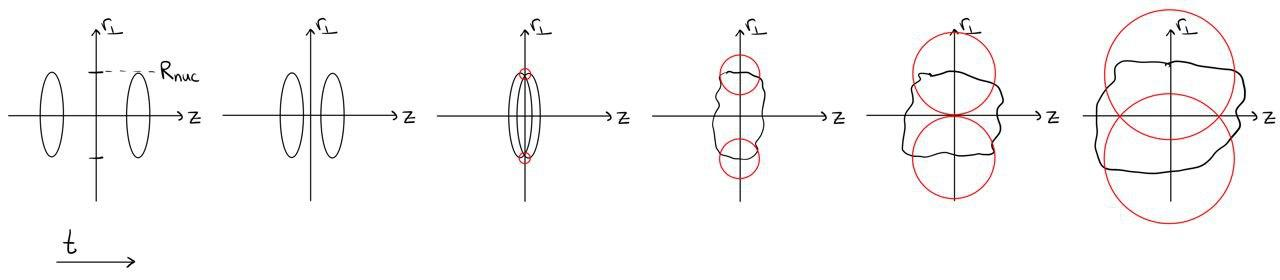
\includegraphics[width=\linewidth]{images/BjorkenFlow_WhatIImagine.jpg}
        \captionof{figure}{At early times the flow at $z\approx 0$ is independent of the extent of the nuclei.}
    \end{minipage}
}
The fluid velocity $u^\mu=(u^\tau, u^{\eta_s},u^\perp)$, assuming only longitudinal flow, takes the form $u^\mu=(1,0,0,0)$.

Baryon conservation reads
\begin{equation}
    0=\nabla_\mu(nu^\mu)=\partial_\mu(nu^\mu)+\Gamma^\mu_{\mu\nu}(nu^\nu)=\partial_\tau n+\frac{n}{\tau}
\end{equation}
The energy-momentum tensor of ideal hydrodynamics in Milne coordinates has components $T^{\tau\tau}=\epsilon$, $T^{\eta_s\eta_s}=\frac{p}{\tau^2}$, $T^{rr}=p$ and $T^{\varphi\varphi}=\frac{p}{r^2}$. Energy-momentum conservation takes the form
\begin{subequations}
    \begin{align}
        0=\nabla_\mu T^{\mu\nu} & =\partial_\mu T^{\mu\nu}+\Gamma^\mu_{\mu\lambda}T^{\lambda\nu}+\Gamma^\nu_{\mu\lambda}\underbrace{T^{\mu\lambda}}_{\text{diagonal}\implies\mu=\lambda}                                          \\
                                & =\partial_\mu T^{\mu\nu}+(\Gamma^{\eta_s}_{\eta_s\tau}T^{\tau\nu}+\Gamma^\varphi_{\varphi r}T^{r\nu})+(\Gamma^\nu_{\eta_s\eta_s}T^{\eta_s\eta_s}+\Gamma^\nu_{\varphi\varphi}T^{\varphi\varphi})
    \end{align}
\end{subequations}
Evaluate different components of this equation
\begin{subequations}
    \begin{align}
        \nu=\tau:    & \qquad 0 =\partial_\tau\epsilon+(\frac{\epsilon}{\tau}+0)+(\tau\frac{p}{\tau^2}+0) \\
        \nu=\eta_s:  & \qquad 0 =\partial_{\eta_s}(\frac{p}{\tau^2})                                      \\
        \nu=r:       & \qquad 0 =\partial_rp+(0+\frac{p}{r})+(0-r^3p)                                     \\
        \nu=\varphi: & \qquad 0 =\partial_\varphi(r^2p)
    \end{align}
\end{subequations}
This implies that $\epsilon=\epsilon(\tau)$ and $p=p(\tau)$ as well as
\begin{equation}
    \partial_\tau\epsilon=-\frac{\epsilon+p}{\tau}
\end{equation}

\done\todo[Only 2 variables are evolved ($\mu,T$) all others follow from algebraic relations of thermodynamics]{The equation of state $p(\epsilon)$ closes the system. But from Legendre trafos, $p$ is a function of $(T,\mu)$? How does hydrodynamics and equilibrium thermodynamics come together? After a hydro simulation, e.g. $\epsilon$ is given as a function of $x$, not of some thermo variable.}

\subsection{Blast Wave Model}

\paragraph*{Basic Idea \cite{JaiswalKoch_2015}}\mbox{}
\begin{itemize}
    \item assume boost-invariant longitudinal flow
    \item assume functional form of phase space density at kinetic freezout \done\todo[Chemical: Interaction that convert the particle species stop. Kinetic: Interactions that keep energy-pressure balance stop]{Find a precise definition of kinetic freezout and also chemical freezout}
    \item parameters: kinetic temperature, radial flow strength, anisotropy in radial flow, source anisotropy
\end{itemize}

Work in Milne coordinates $(\tau,\eta_s,r,\varphi)$.

Boost invariance and rotational symmetry imply $u_\varphi=u_{\eta_s}=0$ \todo[My guess: Boost invariance means $v_z=\frac{z}{t}$, a cube in the fluid moves along straight lines of constant $\eta$]{Why exactly does boost invariance and rotational symmetry imply $u_\varphi=u_{\eta_s}=0$?}\\
\debugbox{
    \begin{minipage}{\linewidth}
        \centering
        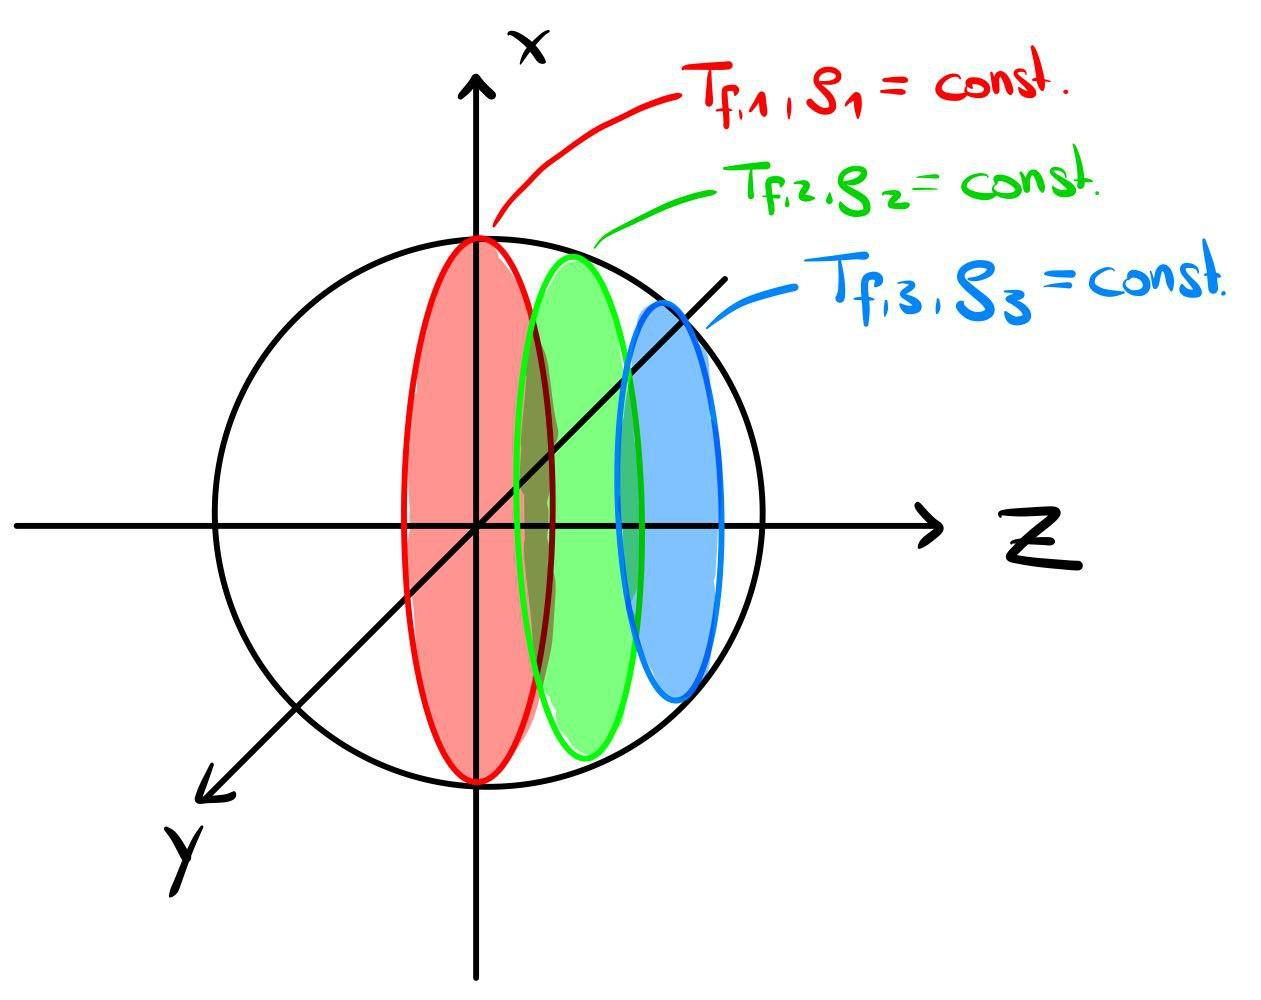
\includegraphics[width=0.5\linewidth]{images/Freezout.jpg}
        \captionof{figure}{Freezout.}
        \todo[At $z=0$ this is correct.]{Is this image correct? Do the planes freezout at the same proper time?}
    \end{minipage}
}
\textbf{Assumptions of the blast-wave model} are that the particle freezout happens at proper time $\tau_f$ when the fluid has constant temperature $T_f$ and uniform matter distribution along the transverse plane
\begin{subequations}
    \begin{align}
        T         & =T_f\Theta(R-r)                \\
        u_r       & =u_0(\frac{r}{R})^n\Theta(R-r) \\
        u_\varphi & =u_{\eta_s}=0                  \\
        u_\tau    & =\sqrt{1+(u_r)^2}
    \end{align}
\end{subequations}
\begin{equation}
    \frac{\dt r}{\dt\tau}=u_0(\frac{r}{R})^n\qquad\implies\qquad\int_{r_0}^R\frac{\dt r}{r^n}=\int_0^{\tau_f}\dt\tau\frac{u_0}{R^n}
\end{equation}
which implies
\begin{equation}
    \frac{\tau_fu_0}{R^n}=
    \begin{cases}
        n=1: & \ln\frac{R}{r_0}                                     \\
        n>1: & \frac{1}{n-1}(\frac{1}{R^{n-1}}-\frac{1}{r_0^{n-1}})
    \end{cases}
\end{equation}
For $n=1$ the radius of the fireball at freezout is given by
\begin{equation}
    R=r_0\exp\left(\frac{u_0\tau_f}{R}\right)
\end{equation}
The freezout time $\tau_f$ can be determined under the assumption of Bjorken flow.
\begin{equation}
    \tau_f=\tau_0\left(\frac{\epsilon_i}{\epsilon_{i0}}\right)^\frac{3}{4}
\end{equation}
where $\epsilon$ is the energy density and the index "$0$" corresponds to central collision.

\subsection{Freezout \cite{DevetakEtAl_2020}}

The hydrodynamic description of the fireball eventually breaks down as the system cools down. Hydro variables (fluid velocity, temperature) are then replaced by hadronic degrees of freedom, i.e. particle spectra.

The Cooper-Frye procedure relates particle spectra to hydro variables via
\begin{equation}
    E_{\mathbf{p}}\frac{\dt N_a}{\dt^3\mathbf{p}}=\frac{\nu_a}{(2\pi)^3}\int_\Sigma\dt\Sigma_\mu p^\mu f_a(\overline{E}_\mathbf{p},T(x),\mu(x))
\end{equation}
\todo[parametrize the momenta with Milne coordinates as Flörchinger sketched it and you will find the equivalence.]{What about this form of the particle spectrum \begin{equation}
        \frac{1}{2\pi p_T}\frac{\dt^2 N}{\dt p_T\dt Y}\Big\vert_{Y=0}=\mathcal{N}\int_0^R\dt rrm_TI_0\left(\frac{p_T\sinh(\artanh u_r)}{T_f}\right)K_1\left(\frac{m_T\cosh(\artanh u_r)}{T_f}\right)
    \end{equation} from \cite{ChenEtAl_2021}?}
with $\overline{E}_\mathbf{p}=p^\mu u_\mu$ the energy in the fluid rest-frame (with fluid velocity $u^\mu$) and $\nu_a$ the spin degeneracy. $f_a$ is a particle distribution function, which depends on the fluid fields $u^\mu(x)$, $T(x)$, $\mu(x)$ and viscious corrections. The distribution function is modelled by the equilibrium Fermi-Dirac- or Bose-Einstein distribution plus corrections due to higher order hydrodynamics
\begin{equation}
    f=f_{\text{eq}}+\delta f_{\text{bulk}}+\delta f_{\text{shear}}
\end{equation}
which take the form
\begin{subequations}
    \begin{align}
        f_{\text{eq}}           & =\frac{1}{\exp(u_\mu p^\mu/T)+s^{(B,F)}} \\
        \delta f_{\text{bulk}}  & =\dots                                   \\
        \delta f_{\text{shear}} & =\dots
    \end{align}
\end{subequations}
where with $s^{(B)}=-1$ and $s^{(F)}=+1$ for Bosons and Fermions respectively. Unstable resonances (particle types) will decay into long-lived particles. These decays can be accounted for already in the distribution function before integrating. This is done numerically with the help of decay precomputable decay kernels \cite{MazeliauskasEtAl_2019}.


\section{Bose-Einstein Condensation}

The partition function in the grand canonical potential is given by
\begin{equation}
    Z=\Tr e^{-\frac{\hat{H}-\mu\hat{N}}{T}}
\end{equation}
For a system with excited states of energy $E_\alpha$ which are occupied by $n_\alpha$ particles the partition becomes
\begin{equation}
    Z=\sum_{n_\alpha}\exp\left(-\frac{1}{T}\sum_\alpha n_\alpha(E_\alpha-\mu)\right)=\prod_\alpha\left[\sum_{n_\alpha}\exp\left(-\frac{1}{T}n_\alpha(E_\alpha-\mu)\right)\right]
\end{equation}
For bosons $n_\alpha\in\mathbb{N}_0$, for fermions $n_\alpha\in\{0,1\}$ and the sums over $n_\alpha$ can be executed as
\begin{subequations}
    \begin{align}
        \text{for bosons:}   &  & \sum_{n_\alpha=0}^\infty \exp\left(-\frac{1}{T}n_\alpha(E_\alpha-\mu)\right) & = \frac{1}{1-\exp(-\frac{E_\alpha-\mu}{T})} \qquad\text{if}\,\mu <E_\alpha\,(\forall\alpha) \\
        \text{for fermions:} &  & \sum_{n_\alpha=0}^1 \exp\left(-\frac{1}{T}n_\alpha(E_\alpha-\mu)\right)      & = 1+\exp(-\frac{E_\alpha-\mu}{T})
    \end{align}
\end{subequations}
Average particle number is then given by
\begin{equation}
    N=T\frac{\partial}{\partial_\mu}\ln Z=T\frac{\partial}{\partial_\mu}\left[\pm\ln\left(\prod_\alpha\left[1\mp\exp\left(-\frac{E_\alpha-\mu}{T}\right)\right]\right)\right]=\sum_\alpha\frac{1}{\exp\left(\frac{E_\alpha-\mu}{T}\right)\mp 1}\equiv\sum_\alpha n_\alpha
\end{equation}
where average occupation number of each level is defined by $n_\alpha$. If the energy levels are independent of the particle spin $s$ and hence have degeneracy $\nu_s=2s+1$ one replaces the sum $\sum_\alpha=\nu_s\sum_{\alpha^\prime}$ where $\alpha^\prime$ label unique single particle energies. The ${\,\cdot\,}^\prime$ is now omitted.
For free particles in $\mathbb{R}^3$ with single particle energies $E=\frac{\mathbf{p}^2}{2m}$ the abstract index $\alpha$ becomes continuous. Take instead a finite box and $\mathbf{x}\in[0,L]^d$. In this scenario momenta are discretized $\mathbf{p}=\frac{2\pi\mathbf{k}}{L}$ with $\mathbf{k}\in\mathbf{Z}^d$. One finds for the discretization $\Delta p_i=\frac{2\pi}{L}\Delta k_i$ with $\Delta k_i=1$ and hence
\begin{equation}
    \sum_\alpha\equiv\sum_{k_1,\dots k_d}\Delta k_1\dots\Delta k_d=\frac{L^d}{(2\pi)^d}\sum_{p_1,\dots p_d}\Delta p_1\dots\Delta p_d\overset{\Delta p_i\to 0}{\to}\int\frac{L^d}{(2\pi)^d}\int\dt^dp
\end{equation}

The thermal particle density in the large volume limit is given by
\begin{equation}
    n_{\text{therm}}(\mu,T)=\nu_s\int\frac{\dt^3p}{(2\pi)^3}\frac{1}{\exp\left(\frac{\mathbf{p}^2/(2m)-\mu}{T}\right)-1}=\frac{\nu_s\pi^\frac{3}{2}(2mT)^\frac{3}{2}}{(2\pi)^3}\text{Li}_\frac{3}{2}(\exp(\frac{\mu}{T}))=\nu_s\left(\frac{mT}{2\pi}\right)^\frac{3}{2}\text{Li}_\frac{3}{2}(\exp(\frac{\mu}{T}))
    \label{eq:BEC_ThermalParticleDensity}
\end{equation}

\begin{impt}[Polylogarithms]{impt:Polylogarithms}
    Define
    \begin{equation}
        \text{Li}_s(z)=\sum_{n=1}^\infty\frac{z^n}{n^s}=\frac{1}{\Gamma(s)}\int_0^\infty\dt\frac{t^{s-1}}{e^tz^{-1}-1}
    \end{equation}
    which also implies
    \begin{equation}
        \frac{1}{\Gamma(s)}\int_0^\infty\dt t\frac{t^{s-1}}{e^tz^{-1}\mp 1}=\pm\text{Li}_s(\pm z)
    \end{equation}
    With this
    \begin{subequations}
        \begin{align}
            \int\dt^dp\frac{1}{\exp(a\mathbf{p}^2)z^{-1}\mp 1} & =\Omega_d\int_0^\infty\dt p\frac{(p^2)^\frac{d-1}{2}}{\exp(ap^2)z^{-1}\mp 1}               \\
            \overset{\substack{t=ap^2                                                                                                                       \\\dt t=2\sqrt{at}\dt p}}&{=}\Omega_d\int_0^\infty\frac{\dt t}{2\sqrt{at}}\frac{a^\frac{1-d}{2}t^\frac{d-1}{2}}{\exp(t)z^{-1}\mp 1}\\
                                                               & =\frac{\Omega_d}{2a^\frac{d}{2}}\int_0^\infty\dt t\frac{t^{\frac{d}{2}-1}}{e^tz^{-1}\mp 1} \\
                                                               & =\pm\frac{\Omega_d\Gamma(\frac{d}{2})}{2a^\frac{d}{2}}\text{Li}_\frac{d}{2}(\pm z)         \\
            \pm                                                & =\frac{\pi^\frac{d}{2}}{a^\frac{d}{2}}\text{Li}_\frac{d}{2}(\pm z)
        \end{align}
    \end{subequations}
    where $\Omega_d=\frac{2\pi^\frac{d}{2}}{\Gamma(\frac{d}{2})}$ was used.
\end{impt}

The chemical potential is restricted to $\mu\leq 0$ and the particle density for fixed temperature is bounded from above by $n_{\text{therm}}<n_{\text{therm}}(\mu\nearrow 0,T)$. However for the ground state of the system $E_\alpha=0$ and the occupation number $n_\alpha$ diverges to $+\infty$ as $\mu\nearrow 0$, indicating macroscopic occupation which changes the description. The critical density for fixed temperature is
\begin{equation}
    n_c=\nu_s\left(\frac{mT}{2\pi}\right)^\frac{3}{2}\zeta(\frac{3}{2})
\end{equation}
or for fixed temperature
\begin{equation}
    T_C=\frac{2\pi}{m}\left(\frac{n}{\nu_s\zeta(\frac{3}{2})}\right)^\frac{2}{3}
\end{equation}
One can think of the critical values as the limits after which the convergence condition $\mu\leq 0$ is not longer satisfied. Alternatively one can ask the question, whether $\mu=0$ is reached for $T>0$ at fixed $n$. For $T\to 0$ it should definitely approach to $0$, since at $T=0$ no particle should occupy an excited state, $n_{\alpha>0}\overset{T\to 0}{\to}0$.

Bose-Einstein condensation appears for $T<T_c$ or $n>n_c$. If $n_0$ is macroscopically large, it is not well described by the integration procedure above. One should rather split the total density into its thermal contribution and the contribution from the ground state,
\begin{equation}
    n=n_0+n_{\text{therm}}
\end{equation}
For fixed $n$ and $T\geq T_C$ $n_0\approx 0$ can be assumed. $n_{\text{therm}}$ is still given by the integral \eqref{eq:BEC_ThermalParticleDensity} and for $T\geq T_C$ equals the total particle density $n$. Hence the macroscopic density in the ground state for $T<T_C$ is given by
\begin{equation}
    n_0=n-n_{\text{therm}}=n\left[1-\left(\frac{T}{T_C}\right)^\frac{3}{2}\right]
\end{equation}

\subsection{Relativistic Bose-Einstein Statistics}

In $d+1$ spacetime dimensions the particle number density
\begin{equation}
    n=\nu_s\int\frac{\dt^dp}{(2\pi)^d}\left[\frac{1}{\exp(\frac{E_{\mathbf{p}}-\mu}{T})-1}-\frac{1}{\exp(\frac{E_{\mathbf{p}}+\mu}{T})-1}\right]
\end{equation}
is the difference between particles and antiparticles. Note $E_{\mathbf{p}}=\sqrt{\mathbf{p}^2+m^2}$. Convergence requires $\abs{\mu}<m$. \done\todo[Yes. This assumes a free gas without interaction vertices. For an interacting theory its different.]{This only includes $1$-loop order corrections to the effective potential.} Note that for $T\ll m$ this reduces to the non-relativistic case, since the second summand/antiparticle contribution becomes negligible.
\begin{subequations}
    \begin{align}
        \frac{1}{\exp(\frac{E_{\mathbf{p}}-\mu}{T})-1}-\frac{1}{\exp(\frac{E_{\mathbf{p}}+\mu}{T})-1} & =\frac{\exp(\frac{E_{\mathbf{p}}+\mu}{T})-\exp(\frac{E_{\mathbf{p}}-\mu}{T})}{\exp(\frac{2E_{\mathbf{p}}}{T})-\exp(\frac{E_{\mathbf{p}}-\mu}{T})-\exp(\frac{E_{\mathbf{p}}+\mu}{T})+1} \\
                                                                                                      & =\frac{\sinh(\frac{\mu}{T})}{\cosh(\frac{E_\mathbf{p}}{T})-\cosh(\frac{\mu}{T})}                                                                                                       \\
                                                                                                      & =\frac{\exp(\frac{E_{\mathbf{p}}}{T})(2\frac{\mu}{T}+\mathcal{O}(\frac{\mu}{T})^2)}{(\exp(\frac{E_{\mathbf{p}}}{T})+1)^2+\mathcal{O}(\frac{\mu}{T})^2}
    \end{align}
\end{subequations}
and hence
\begin{equation}
    n=\nu_s\frac{\Omega_{d}}{(2\pi)^d}\int_0^\infty\dt pp^{d-1}\frac{\sinh(\frac{\mu}{T})}{\cosh(\frac{E_\mathbf{p}}{T})-\cosh(\frac{\mu}{T})}=\nu_s\frac{2\pi^\frac{d}{2}}{\Gamma(\frac{d}{2})(2\pi)^d}\int_0^\infty\dt pp^{d-1}\frac{\sinh(\frac{\mu}{T})}{\cosh(\frac{E_\mathbf{p}}{T})-\cosh(\frac{\mu}{T})}
\end{equation}

What is $\lim_{x\to0}\frac{x^b}{\cosh\sqrt{x^2+a^2}-\cosh a}$? ($b>0$)
\begin{subequations}
    \begin{align}
        \lim_{x\to0}\frac{x^b}{\cosh\sqrt{x^2+a^2}-\cosh a} & =\lim_{x\to0}\frac{bx^{b-1}}{\sinh(\sqrt{x^2+a^2})\frac{x}{\sqrt{x^2+a^2}}} \\
                                                            & =\lim_{x\to0}\frac{bx^{b-2}\sqrt{x^2+a^2}}{\sinh\sqrt{x^2+a^2}}
        \begin{cases}
            =0                            & \iff\quad b\geq 2 \\
            \text{diverges with}\,x^{b-2} & \iff\quad b<2
        \end{cases}
    \end{align}
\end{subequations}
For $a=0$ one can instead expand $\cosh(x)=1+\mathcal{O}(x^2)$ and find the same criterion.

The critical values of density or temperature are now found by setting $\abs{\mu}=m$. Further assume $T\gg m$. Then the integral converges if $d-1>1$ (the integration improves convergence by 1 order) and we find for $d=3$ \todo{Check exactly what the error is for the $p\to 0$ contribution of this integral.}
\begin{equation}
    \abs{n}=\nu_s\frac{2\pi^\frac{3}{2}}{\Gamma(\frac{3}{2})(2\pi)^3}\frac{2m}{T}\int_0^\infty\dt pp^2\frac{\exp(\frac{p}{T})}{(\exp(\frac{p}{T})+1)^2}=\frac{1}{\frac{\sqrt{\pi}}{2}\pi^\frac{3}{2}}\frac{m}{T}T^3\int_0^\infty\dt xx^2\frac{e^x}{(e^x+1)^2}=\frac{2mT^2}{\pi^2}\frac{\pi^2}{6}=\frac{mT^2}{3}
\end{equation}
implying (if $T\gg m$ or $\abs{n}\gg m^3$)
\begin{subequations}
    \begin{align}
        \abs{n_c} & =\frac{mT^2}{3}                                \\
        T_c       & =\left(\frac{3\abs{n}}{m}\right)^{\frac{1}{2}} \\
        \intertext{and if $m\ll T<T_c$}
        n_0       & =n\left[1-\left(\frac{T}{T_c}\right)^2\right]
    \end{align}
\end{subequations}
The general result in $d+1$ spacetime dimensions in the ultrarelativistic limit is \cite{GretherEtAl_2007}
\begin{equation}
    T_c^{UR}=\left[\frac{\Gamma(\frac{d}{2})(2\pi)^d}{4m\pi^\frac{d}{2}\Gamma(d)\zeta(d-1)}\right]^\frac{1}{d-1}n^\frac{1}{d-1}
\end{equation}

The energy of a particle with 4-momentum $p^\mu$ measured from an observer with 4-velocity $u^\mu$ is $E_{\mathbf{p}}=p^\mu u_\mu$ and we get
\begin{align}
    n=\nu_s\int\frac{\dt^{d-1}p}{(2\pi)^{d-1}}\left[\frac{1}{\exp(\frac{p^\mu u_\mu-\mu}{T})-1}-\frac{1}{\exp(\frac{p^\mu u_\mu+\mu}{T})-1}\right]
\end{align}




\section{Particle Physics and Group Theory}

\subsection{Isospin}

It is found that $m_{\text{proton}}\approx m_{\text{neutron}}$. Take this as a motivation to represent proton and neutron as 2 states of a single entity, just as $\ket{\uparrow}$ and $\ket{\downarrow}$ are basis states for a spin-$\frac{1}{2}$ particle.
\begin{equation}
    \ket{p}=\begin{pmatrix}
        1 \\0
    \end{pmatrix}\,,
    \qquad
    \ket{n}=\begin{pmatrix}
        0 \\1
    \end{pmatrix}
\end{equation}
The transformations acting on these states are supposed to be unitary. Neglecting phase factors the corresponding symmetry group is $SU(2)$. The above state form a douplet under \textbf{isospin} transformations with total isospin $I=\frac{1}{2}$ and third component $I_3=\pm\frac{1}{2}$. This idea is extend to up-/down-quarks or up-/down-/strange-quarks since $m_u\approx m_d\approx m_s$.
\begin{equation}
    \ket{u}=\begin{pmatrix}
        1 \\0\\0
    \end{pmatrix}\,,\qquad
    \ket{d}=\begin{pmatrix}
        0 \\1\\0
    \end{pmatrix}\,,\qquad
    \ket{s}=\begin{pmatrix}
        0 \\0\\1
    \end{pmatrix}
\end{equation}
The corresponding symmetry neglecting phase factors is $SU(3)$ with 8 generators $T_i$. \done\todo[Isospin is $SU(2)$ betweend $u$ and $d$ or $p$ and $n$. For $u,d,s$ we would call it flavor symmetry.]{Is isospin the same is flavor symmetry?}

\subsection{Representations of $SU(3)$}

The $\mathbf{3}$-representation or fundamental representation is given by $T_i=\frac{1}{2}\lambda_i$ with the Gell-Mann matrices $\lambda_i$. They constructed as follows: Choose the first three to reflect ud-symmetry ($\to SU(2)$)
\begin{subequations}
    \begin{align}
        \lambda_1=\begin{pmatrix}
            0 & 1 & 0 \\
            1 & 0 & 0 \\
            0 & 0 & 0
        \end{pmatrix}\,,\qquad
        \lambda_2=\begin{pmatrix}
            0      & -\imagu & 0 \\
            \imagu & 0       & 0 \\
            0      & 0       & 0
        \end{pmatrix}\,,\qquad
        \lambda_3=\begin{pmatrix}
            1 & 0  & 0 \\
            0 & -1 & 0 \\
            0 & 0  & 0
        \end{pmatrix}        \\
        \intertext{This construction is mirrored to reflect us- and ds-symmetry}
        \lambda_4=\begin{pmatrix}
            0 & 0 & 1 \\
            0 & 0 & 0 \\
            1 & 0 & 0
        \end{pmatrix}\,,\qquad
        \lambda_5=\begin{pmatrix}
            0      & 0 & -\imagu \\
            0      & 0 & 0       \\
            \imagu & 0 & 0       \\
        \end{pmatrix}\,,\qquad
        \lambda_8^\prime=\begin{pmatrix}
            1 & 0 & 0  \\
            0 & 0 & 0  \\
            0 & 0 & -1
        \end{pmatrix} \\
        \lambda_6=\begin{pmatrix}
            0 & 0 & 0 \\
            0 & 0 & 1 \\
            0 & 1 & 0
        \end{pmatrix}\,,\qquad
        \lambda_7=\begin{pmatrix}
            0 & 0      & 0       \\
            0 & 0      & -\imagu \\
            0 & \imagu & 0
        \end{pmatrix}\,,\qquad
        \lambda_8^{\prime\prime}=\begin{pmatrix}
            0 & 0 & 0  \\
            0 & 1 & 0  \\
            0 & 0 & -1
        \end{pmatrix}
    \end{align}
    Note that only one of $\lambda_8^\prime,\lambda_8^{\prime\prime}$ can be linearly independent. One instead chooses
    \begin{equation}
        \lambda_8=\frac{1}{\sqrt{3}}(\lambda_8^\prime+\lambda_8^{\prime\prime})=\frac{1}{\sqrt{3}}\begin{pmatrix}
            1 & 0 & 0  \\
            0 & 1 & 0  \\
            0 & 0 & -2
        \end{pmatrix}
    \end{equation}
    \label{eq:GroupTheory_SU3_FundRep}
\end{subequations}
Alternatively define
\begin{equation}
    I_\pm=T_1\pm\imagu T_2\,,\qquad V_\pm=T_4\pm\imagu T_5\,,\qquad U_\pm=T_6\pm\imagu T_7
\end{equation}
A basis of $\mathfrak{su}(3)$ is given by $\{T_i\}$ or $\{I_\pm,V_\pm,U_\pm,T_3,T_8\}$. The algebra has two \textbf{Casimir operators}
\begin{equation}
    C_2=\sum_{j=1}^8T_j^2\,,\qquad C_3=\sum_{j,k,l=1}^8T_j^2
\end{equation}
that commute with all operators and hence all states can be labelled by 2 labels. Since $[T_3,T_8]=0$ use the eigenstates $\ket{i_3,i_8}$ such that
\begin{equation}
    T_3\ket{i_3,i_8}=i_3\ket{i_3,i_8}\,,\qquad T_8\ket{i_3,i_8}=i_8\ket{i_3,i_8}
\end{equation}
The ladder operators act as
\begin{subequations}
    \begin{align}
        I_\pm\ket{i_3,i_8} & \propto\ket{i_3\pm 1,i_8}                                \\
        V_\pm\ket{i_3,i_8} & \propto\ket{i_3\pm \frac{1}{2},i_8\pm\frac{\sqrt{3}}{2}} \\
        U_\pm\ket{i_3,i_8} & \propto\ket{i_3\mp \frac{1}{2},i_8\pm\frac{\sqrt{3}}{2}}
    \end{align}
\end{subequations}

\debugbox{
    \begin{minipage}{\linewidth}
        \centering
        \begin{tikzpicture}[scale=2]
            \draw[->] (-1.5,0) -- (1.5,0) node[right]{$i_3$};
            \draw[->] (0,-1.5) -- (0,1.5) node[above]{$i_8$};

            \draw[thick,->] (0,0) -- (1,0) node[below]{$\mathbf{I}_+$};
            \draw[thick,->] (0,0) -- (-1,0) node[below]{$\mathbf{I}_-$};

            \draw[thick,->] (0,0) -- (0.5,{sqrt(3)/2}) node[above]{$\mathbf{V}_+$};
            \draw[thick,->] (0,0) -- (-0.5,-{sqrt(3)/2}) node[below]{$\mathbf{V}_-$};

            \draw[thick,->] (0,0) -- (0.5,-{sqrt(3)/2}) node[below]{$\mathbf{U}_-$};
            \draw[thick,->] (0,0) -- (-0.5,{sqrt(3)/2}) node[above]{$\mathbf{U}_+$};
        \end{tikzpicture}
    \end{minipage}
}

One can read off
\begin{equation}
    \ket{u}=\ket{\frac{1}{2},\frac{1}{2\sqrt{3}}}\,,\qquad\ket{d}=\ket{-\frac{1}{2},\frac{1}{2\sqrt{3}}}\,,\qquad\ket{s}=\ket{0,-\frac{1}{\sqrt{3}}}
\end{equation}
and the ladder operators act as
\begin{subequations}
    \begin{align}
         &  & V_-\ket{u} & \propto\ket{s}\,, & V_+\ket{s} & \propto\ket{u} &  & \\
         &  & I_-\ket{u} & \propto\ket{d}\,, & I_+\ket{d} & \propto\ket{u} &  & \\
         &  & U_-\ket{d} & \propto\ket{s}\,, & U_+\ket{s} & \propto\ket{d} &  &
    \end{align}
\end{subequations}
The states are represented diagrammatically\\
\debugbox{
    \begin{minipage}{\linewidth}
        \centering
        \begin{tikzpicture}[scale=2]
            \draw[->] (-1.5,0) -- (1.5,0) node[right]{$i_3$};
            \draw[->] (0,-1.5) -- (0,1.5) node[above]{$i_8$};

            \coordinate[label=45:{$u$}] (u) at (0.5,{1/(2*sqrt(3))});
            \coordinate[label=135:{$d$}] (d) at (-0.5,{1/(2*sqrt(3))});
            \coordinate[label=45:{$s$}] (s) at (0,-{1/(sqrt(3))});

            \draw[fill] (u) circle (0.05);
            \draw[fill] (d) circle (0.05);
            \draw[fill] (s) circle (0.05);
        \end{tikzpicture}
    \end{minipage}
}

Define charge conjugated generators via
\begin{equation}
    T_j^C\defeq -T_j^*\overset{T_j=T_j^\dagger}{=}-T_j^T
\end{equation}
The sign in this definition ensures
\begin{equation}
    [T_j^C,T_k^C]=\imagu f_{jkl}T_l^C
\end{equation}

It is obvious that $T_{2,5,7}^C=T_{2,5,7}$ and $T_{1,3,4,6,8}^C=-T_{1,3,4,6,8}$, hence the charge conjugation operator $\mathcal{C}$ acts on the basis states as
\begin{equation}
    \mathcal{C}\ket{i_3,i_8}=\ket{-i_3,-i_8}
\end{equation}
This defines the charge conjugate representation $\mathbf{3}^*$ with the basis
\begin{equation}
    \ket{\overline{u}}=\ket{-\frac{1}{2},-\frac{1}{2\sqrt{3}}}\,,\qquad\ket{\overline{d}}=\ket{\frac{1}{2},-\frac{1}{2\sqrt{3}}}\,,\qquad\ket{\overline{s}}=\ket{0,-\frac{1}{\sqrt{3}}}
\end{equation}

The \textbf{adjoint representation} is defined by linearly mapping the generators to linear maps on the generators via the Lie bracket,
\begin{equation}
    \text{adj}(T_j)X=[T_j,X]
\end{equation}
Consider $X=x_kT_k$ to find the matrix elements $[\text{adj}(T_j)]_{ab}$ that fulfill $x_l^\prime=[\text{adj}(T_j)]_{lk}x_k$ if $\text{adj}(T_j)X=X^\prime$.
\begin{equation}
    [\text{adj}(T_j)]_{lk}x_kT_l=\text{adj}(T_j)X=x_k[T_j,T_k]=\imagu f_{jkl}x_kT_l\qquad\iff\qquad[\text{adj}(T_j)]_{lk}=\imagu f_{jkl}
\end{equation}
The Jacobi identity of the representation $\{T_j\}$ ensures
\begin{equation}
    [\text{adj}(T_j),\text{adj}(T_k)]X=\text{adj}([T_j,T_k])X\equiv \imagu f_{jkl}\text{adj}(T_l)X
\end{equation}
such that the adjoint representation is in fact a representation of the same algebra. The corresponding states are now the generators themselves \todo{It doesn't matter of which representation one thinks about the states, right? There are no different adjoint representations. Still, the eigenvalues depend on the precise choice of basis we did at the beginning} \todo{Why are exactly the ladder operators the correct eigenstates?}

\debugbox{
    \begin{minipage}{\linewidth}
        \centering
        \begin{tikzpicture}[scale=2]
            \draw[->] (-1.5,0) -- (1.5,0) node[right]{$i_3$};
            \draw[->] (0,-1.5) -- (0,1.5) node[above]{$i_8$};

            \coordinate[label=120:{$U_+$}] (Up) at (-0.5,{sqrt(3)/2});
            \coordinate[label=-60:{$U_-$}] (Um) at (0.5,-{sqrt(3)/2});
            \coordinate[label=120-60:{$V_+$}] (Vp) at (0.5,{sqrt(3)/2});
            \coordinate[label=-60-60:{$V_-$}] (Vm) at (-0.5,-{sqrt(3)/2});
            \coordinate[label=60:{$I_+$}] (Ip) at (+1,0);
            \coordinate[label=120:{$I_-$}] (Im) at (-1,0);
            \coordinate[label=60:{$T_8$}] (T8) at (0.05,0);
            \coordinate[label=120:{$T_3$}] (T3) at (-0.05,0);

            \draw[fill] (Up) circle (0.05);
            \draw[fill] (Um) circle (0.05);
            \draw[fill] (Vp) circle (0.05);
            \draw[fill] (Vm) circle (0.05);
            \draw[fill] (Ip) circle (0.05);
            \draw[fill] (Im) circle (0.05);
            \draw[fill] (T8) circle (0.05);
            \draw[fill] (T3) circle (0.05);

        \end{tikzpicture}
    \end{minipage}
}

Study now the tensor product representation $\mathbf{3}\otimes\mathbf{3}$ with a basis $\{\ket{i_3i_8}\otimes\ket{j_3j_8}\}$ with $i,j$ the quantum numbers of two copies of $\mathfrak{su}(3)$. Corresponding operators are defined by $T=T^{(1)}+T^{(2)}$ and the eigenvalues of the tensor product space are sums of the eigenvalues in the two copies.\\
\debugbox{
    \begin{minipage}{\linewidth}
        \centering
        \begin{tikzpicture}[scale=2]
            \draw[->] (-1.5,0) -- (1.5,0) node[right]{$i_3$};
            \draw[->] (0,-1.5) -- (0,1.5) node[above]{$i_8$};

            \coordinate (u) at (0.5,{1/(2*sqrt(3))});
            \coordinate (d) at (-0.5,{1/(2*sqrt(3))});
            \coordinate (s) at (0,-{1/(sqrt(3))});

            \coordinate[label=30:{$uu$}] (uu) at ($(u)+(u)$);
            \coordinate[label=150:{$dd$}] (dd) at ($(d)+(d)$);
            \coordinate[label=30:{$ss$}] (ss) at ($(s)+(s)$);
            \coordinate[label=30:{$du$}] (du) at ($(d)+(u)+(0.05,0)$);
            \coordinate[label=150:{$ud$}] (ud) at ($(u)+(d)-(0.05,0)$);
            \coordinate[label=30:{$su$}] (su) at ($(s)+(u)+(0.05,0)$);
            \coordinate[label=150:{$us$}] (us) at ($(u)+(s)-(0.05,0)$);
            \coordinate[label=30:{$ds$}] (ds) at ($(d)+(s)+(0.05,0)$);
            \coordinate[label=150:{$sd$}] (sd) at ($(s)+(d)-(0.05,0)$);

            \draw (u) circle (0.05);
            \draw (d) circle (0.05);
            \draw (s) circle (0.05);

            \draw[fill] (uu) circle (0.05);
            \draw[fill] (dd) circle (0.05);
            \draw[fill] (ss) circle (0.05);
            \draw[fill] (ud) circle (0.05);
            \draw[fill] (du) circle (0.05);
            \draw[fill] (us) circle (0.05);
            \draw[fill] (su) circle (0.05);
            \draw[fill] (ds) circle (0.05);
            \draw[fill] (sd) circle (0.05);
        \end{tikzpicture}
    \end{minipage}
}
The highest weight state gets annihilated by all of $\{U_+,V_+,I_+\}$. It is therefore $u\otimes u$. \todo{So just like addition of angular momenta it has the highest eigenvalues for the Casimirs?} Applying ladder operators to $u\otimes u$ one finds the representation $\mathbf{6}$ of $\mathfrak{su}(3)$ given by
\begin{subequations}
    \begin{align}
         &  & u\otimes u & =\ket{1,\frac{1}{\sqrt{3}}}\,,  & \frac{1}{\sqrt{2}}(u\otimes d+d\otimes u) & =\ket{0,\frac{1}{\sqrt{3}}}             &  & \\
         &  & d\otimes d & =\ket{-1,\frac{1}{\sqrt{3}}}\,, & \frac{1}{\sqrt{2}}(u\otimes s+s\otimes u) & =\ket{\frac{1}{2},-\frac{1}{2\sqrt{3}}} &  & \\
         &  & s\otimes s & =\ket{0,-\frac{2}{\sqrt{3}}}\,, & \frac{1}{\sqrt{2}}(d\otimes s+s\otimes d) & =\ket{-\frac{1}{2},\frac{1}{2\sqrt{3}}} &  & \\
    \end{align}
\end{subequations}

The missing states to form a basis are
\begin{subequations}
    \begin{align}
        \frac{1}{\sqrt{2}}(d\otimes u-u\otimes d) & =\ket{0,\frac{1}{\sqrt{3}}}             \\
        \frac{1}{\sqrt{2}}(s\otimes u-u\otimes s) & =\ket{\frac{1}{2},-\frac{1}{2\sqrt{3}}} \\
        \frac{1}{\sqrt{2}}(s\otimes d-d\otimes s) & =\ket{-\frac{1}{2},\frac{1}{2\sqrt{3}}} \\
    \end{align}
\end{subequations}
manifesting the $\mathbf{3}^*$ representation. \todo{The bra-ket notation at this point is probably incomplete...there is the quantum number of the Casimir operator missing} In this sense one decomposes $\mathbf{3}\otimes\mathbf{3}=\mathbf{6}\oplus\mathbf{3}^*$. Analogously $\mathbf{3}^*\otimes\mathbf{3}^*=\mathbf{6}^*\oplus\mathbf{3}$. One further finds $\mathbf{3}\otimes\mathbf{3}^*=\mathbf{8}\oplus\mathbf{1}$ and $\mathbf{3}\otimes\mathbf{3}\otimes\mathbf{3}=\mathbf{10}\oplus\mathbf{8}\oplus\mathbf{8}\oplus\mathbf{1}$ where $\mathbf{10}$ has all totally symmetric and $\mathbf{1}$ all totally anti-symmetric states. The states in $\mathbf{3}\otimes\mathbf{3}^*$ are called mesons and those in $\mathbf{3}\otimes\mathbf{3}\otimes\mathbf{3}$ baryons.

Additionally one imposes and additional $SU(3)_C$ color symmetry. It is assumed that all observable states are color neutral and hence singlets under $SU(3)_C$. There are no singlets in $\mathbf{3}\otimes\mathbf{3}\otimes\mathbf{3}^*$ or $\mathbf{3}\otimes\mathbf{3}$ and hence no states corresponding to these representations. \done[It is true that for a symmetry group $S$ that $D_1(S)\otimes D_2(S)$ gives a new valid representation $D_3(S)$, but the representation belong to the same group. On this one cannot simply multiply representations of different groups.]\todo{Why is color symmetry not just an additional $\otimes\mathbf{3}_C$}

Quantum numbers are
\begin{align*}
    B:\qquad     & \text{baryon number}                                                               \\
    S:\qquad     & \text{strangeness, \# of }\overline{s}\text{-quarks }-\text{\# of }s\text{-quarks} \\
    J:\qquad     & \text{spin}                                                                        \\
    I_3:\qquad   & 3\text{-component of isospin}                                                      \\
    Y=B+S:\qquad & \text{hypercharge}
\end{align*}
\todo{Why these quantum numbers? I would have expected 1 isospin and 1 z-component for each particle...}

\done\todo[Yes, one could introduce composite fields for example by means of Hubbard Stratonovich. Alternatively one could keep elementary quark fields and look for bound states by investigating correlation functions on the lattice.]{In general, does each particle type have a different field in the QFT?}


\subsection{From a Field Theory Perspective}

Consider $N_f$ flavors of quarks and the Lagrangian
\begin{equation}
    \mathscr{L}=\overline{\psi}_a(\imagu\gamma^\mu(\partial_\mu+\imagu gA_\mu)-m)\psi^a
\end{equation}
which is invariant under the $SU(N_f)$ transformation
\begin{equation}
    \psi\to U\psi\,,\qquad\overline{\psi}\to\overline{\psi}U^\dagger
\end{equation}
where $UU^\dagger=U^\dagger U=\mathbf{1}$ or $U^a_{\phantom{a}b}(U^\dagger)^b_{\phantom{b}c}=(U^\dagger)^a_{\phantom{a}b}U^b_{\phantom{b}c}=\delta^a_c$. Unitary transformations are written as $U=\exp(-\imagu \alpha^jT_j)$ with $T_j^\dagger T_j=T_jT_j^\dagger=\mathbf{1}$ and $\Tr(T_j)=0$. The hermitian traceless matrices $T_j$ are generators of the algebra $\mathfrak{su}(N_f)$. In terms of generators
\begin{equation}
    U^a_{\phantom{a}b}\approx\delta^a_b-\imagu\alpha_j(T_j)^a_{\phantom{a}b}
\end{equation}
such that
\begin{equation}
    \delta\psi^a=-\imagu\alpha_j(T_j)^a_{\phantom{a}b}\psi^b\,,\qquad\delta\overline{\psi}_a=\imagu\alpha_j\overline{\psi}_b(T_j)^b_{\phantom{b}a}
\end{equation}
By virtue of Noethers theorem the current
\begin{equation}
    j^A_\mu(x)=-\imagu\frac{\partial\mathscr{L}}{\partial(\partial^\mu\psi^a)}(T^A)^a_{\phantom{a}b}\psi^b=\overline{\psi}_a\gamma_\mu(T^A)^a_{\phantom{a}b}\psi^b
\end{equation}
is conserved, $\partial^\mu j_\mu^A=0$. Conserved charges are
\begin{equation}
    Q^A=\int\dt^3x j_0^A(x)
\end{equation}
meaning they commute with the generator of time evolution
\begin{equation}
    [H,Q^A]=0
\end{equation}
and fulfill the $\mathfrak{su}(N_f)$ algebra. \todo{Commutation is then related to the commutation of operator valued fields?} \todo{A state $\ket{\dots}$ is some functional of the field. Acting with $Q^A$ on the state means applying the $\hat{\psi}$\dots operators to this functional?}

\section{Chiral Symmetry}


Consider $N_f$ flavors of quarks and the Lagrangian
\begin{equation}
    \mathscr{L}=\overline{\psi}_a(\imagu\gamma^\mu(\partial_\mu+\imagu gA_\mu)-m)\psi^a=\overline{\psi}_a(\imagu\slashed{D}-m)\psi^a
\end{equation}
where the flavor index $a=1,\dots N_f$ is implicitly summed over and $\overline{\psi}=\psi^\dagger\gamma_0$. Define $\gamma_5$-matrix via
\begin{equation}
    \gamma_5=\imagu\gamma_0\gamma_1\gamma_2\gamma_3
\end{equation}
Thus $\{\gamma_5,\gamma_\mu\}=0$ and $(\gamma_5)^2=\mathbf{1}_{2\times 2}$.
\begin{equation}
    \begin{split}
        (\gamma_5)^2&=-\gamma_0\gamma_1\gamma_2\gamma_3\gamma_0\gamma_1\gamma_2\gamma_3\\
        &=(\gamma_0)^2\gamma_1\gamma_2\gamma_3\gamma_1\gamma_2\gamma_3\\
        &=(\gamma_0)^2(\gamma_1)^2\gamma_2\gamma_3\gamma_2\gamma_3\\
        &=-\prod(\gamma_\mu)^2\\
        &=\mathbb{1}_{2\times 2}
    \end{split}
\end{equation}

Consider now the transformations
\begin{subequations}
    \begin{align}
        U(1)_V & :\qquad \psi\to e^{\imagu\alpha}\psi\,,\quad\overline{\psi}\to e^{-\imagu\alpha}\overline{\psi}               \\
        U(1)_A & :\qquad \psi\to e^{\imagu\alpha\gamma_5}\psi\,,\quad\overline{\psi}\to\overline{\psi}e^{\imagu\alpha\gamma_5}
    \end{align}
    \label{eq:ChiralSymmetry_U1VectorAxial}
\end{subequations}
These are symmetries of the Lagrangian except for the axial symmetry $U(1)_A$ in the case of non-vanishing masses. We wish to apply Noethers theorem
\begin{equation}
    \delta\mathscr{L}=\partial_\mu\left(\frac{\partial\mathscr{L}}{\partial(\partial_\mu\phi)}\delta\phi\right)
\end{equation}
The corresponding Noether currents $J^\mu=-\frac{\partial\mathscr{L}}{\partial(\partial_\mu\psi)}\delta\psi$ are
\begin{subequations}
    \begin{align}
        U(1)_V & :\qquad J^\mu=\overline{\psi}_a\gamma^\mu\psi^a\,,\quad\partial_\mu J^\mu=0                                                \\
        U(1)_A & :\qquad J^\mu=\overline{\psi}_a\gamma^\mu\gamma_5\psi^a\,,\quad\partial_\mu J^\mu=2\imagu m\overline{\psi}_a\gamma_5\psi^a
    \end{align}
\end{subequations}

The symmetry is explicitly written out if one uses projectors
\begin{equation}
    P_\pm=\frac{1\pm\gamma_5}{2}
\end{equation}
that satisfy
\begin{equation}
    \begin{split}
        P_\pm P_\pm=P_\pm\,,\qquad P_\pm P_\mp=0\\
        P_++P_-=1\,,\qquad
        P_\pm\gamma^\mu=\gamma^\mu P_\mp
    \end{split}
\end{equation}
The Lagrangian is then decomposed as
\begin{equation}
    \mathscr{L}=\overline{\psi}_a(\imagu\slashed{D}-m)(P_+^2+P_-^2)\psi^a=(\overline{\psi}_{a+}\imagu\slashed{D}\psi_+^a+\overline{\psi}_{a-}\imagu\slashed{D}\psi_-^a)-m(\overline{\psi}_{a-}\psi_+^a+\overline{\psi}_{a+}\psi_-^a)
\end{equation}
where the projections \todo{Is $\gamma_5$ hermitian?}
\begin{equation}
    \psi_\pm=P_\pm\psi\,,\qquad\overline{\psi}_\pm=\psi^\dagger_\pm\gamma_0=\overline{\psi}P_\mp
\end{equation}
twhere used. Using $\gamma_5=P_+-P_-$ The symmetry transformations \eqref{eq:ChiralSymmetry_U1VectorAxial} in terms of the projections take the form
\begin{subequations}
    \begin{align}
        U(1)_V & :\qquad \psi_\pm\to e^{\imagu\alpha}\psi_\pm\,,\quad\overline{\psi}_\pm\to e^{-\imagu\alpha}\overline{\psi}_\pm      \\
        U(1)_A & :\qquad \psi_\pm\to e^{\pm\imagu\alpha}\psi_\pm\,,\quad\overline{\psi}_\pm\to e^{\mp\imagu\alpha}\overline{\psi}_\pm
    \end{align}
\end{subequations}
Performing simultaneous vector and axial transformations by angles $\alpha_V$ and $\alpha_A$ it follows that $\psi_\pm\to\exp(\imagu[\alpha_V\pm\alpha_A])\psi_\pm\equiv\exp(\imagu\beta_\pm)\psi_\pm$. On this level, it is obvious that
\begin{equation}
    U(1)_V\times U(1)_A=U(1)_+\times U(1)_-
\end{equation}
Note how this symmetry is part of the larger $U(N_f)_+\times U(N_f)_-$. One can use
\begin{equation}
    U(N_f)=(SU(N_f)\times U(1))/\mathbf{Z}_{N_f}
\end{equation}
The quotient is due to the fact that all elements $\exp(k\frac{2\pi\imagu}{N_f})$ with $k\in\{0,1,\dots N_f-1\}$ viewed as $N_f\times N_f$ matrices are $\in SU(N_f)$, thus the mapping $SU(N_f)\times U(1)\to U(N_f)$ is not injective.
The full symmetry group is
\begin{equation}
    SU(N_f)_V\times SU(N_f)_A\times U(1)_V\times U(1)_A
\end{equation}
\todo[I guess $U(1)_A$ is somehow reconstructed from $U(1)_V$ and $SU(N_f)_A$?]{Tong omits the $U(1)_A$, why?} The corresponding transformations take the form
\begin{subequations}
    \begin{align}
        SU(N_f)_+\times U(1)_+ & :\qquad\psi_+^a\to e^{\imagu\alpha_+}(U_+)^a_{\phantom{a}b}\psi_+^b\,,\qquad\overline{\psi}_{+a}\to e^{-\imagu\alpha_+}\overline{\psi}_{+b}(U_+^\dagger)^b_{\phantom{b}a} \\
        SU(N_f)_-\times U(1)_- & :\qquad\psi_-^a\to e^{\imagu\alpha_-}(U_-)^a_{\phantom{a}b}\psi_-^b\,,\qquad\overline{\psi}_{-a}\to e^{-\imagu\alpha_-}\overline{\psi}_{-b}(U_-^\dagger)^b_{\phantom{b}a}
    \end{align}
\end{subequations}

For the vector symmetry $\alpha_+=\alpha_-$ and $U_+=U_-$, and for the axial symmetry $\alpha_+=-\alpha_-$ and $U_+=U_-^\dagger$. \todo[Since the generators are hermitian $U_+=U^\dagger_-$ translates to $\alpha_{+j}=-\alpha_{-j}$]{How does $U(N>1)$ vector/axial symmetry really look like in terms of $\gamma_5$?}
\begin{subequations}
    \begin{align}
        U(N_f)_V & :\qquad\psi^a\to (e^{\imagu\alpha_jT_j})^a_{\phantom{a}b}\psi^b\,,\qquad\overline{\psi}_b\to \overline{\psi}_b(e^{-\imagu\alpha_jT_j})^b_{\phantom{b}a}                \\
        U(N_f)_A & :\qquad\psi^a\to (e^{\imagu\gamma_5\alpha_jT_j})^a_{\phantom{a}b}\psi^b\,,\qquad\overline{\psi}_b\to \overline{\psi}_b(e^{\imagu\gamma_5\alpha_jT_j})^b_{\phantom{b}a}
    \end{align}
\end{subequations}
The conserved currents are simply
\begin{subequations}
    \begin{align}
        U(N_f)_V & :\qquad J^\mu_j=\overline{\psi}_a(T_j)^a_{\phantom{a}b}\gamma^\mu\psi^a\,,\quad\partial_\mu J^\mu=0                                                                        \\
        U(N_f)_A & :\qquad J^\mu_j=\overline{\psi}_a(T_j)^a_{\phantom{a}b}\gamma^\mu\gamma_5\psi^a\,,\quad\partial_\mu J^\mu_j=2\imagu m\overline{\psi}_a(T_j)^a_{\phantom{a}b}\gamma_5\psi^b
    \end{align}
\end{subequations}

\subsection{Unequal Flavor Masses}

If the fermion flavors have different masses $m^{(a)}$ such that
\begin{equation}
    m\sum_a(\overline{\psi}_{a-}\psi_+^a+\overline{\psi}_{a+}\psi_-^a)\to\sum_am^{(a)}(\overline{\psi}_{a-}\psi_+^a+\overline{\psi}_{a+}\psi_-^a)
\end{equation}
then, additionally to the broken axial symmetry, vector symmetry is further broken down
\begin{equation}
    SU(N_f)_V\times U(1)_V\to U(1)^{N_f}
\end{equation}

\subsection{Quark Condensate}

\subsubsection{Non-Linear $\sigma$-Model}

A condensate of the form
\begin{equation}
    \langle\overline{\psi}_{-a}\psi_+^b\rangle=-\sigma\delta_a^b
\end{equation}
breaks axial chiral symmetry spontaneously, denoted as $\chi SB$ ("chiral symmetry breaking"). \done\todo[Solved, see the following]{Why exactly is the manifold of all possible vacua described by $\langle\overline{\psi}_{-a}\psi^b_+\rangle=-\sigma U_a^{\phantom{a}b}$ with $U\in SU(N_f)$?} It transforms according to
\begin{equation}
    \langle\overline{\psi}_{-a}\psi_+^b\rangle\to\langle\overline{\psi}_{-c}(U^\dagger_-)^c_{\phantom{c}a}(U_+)^b_{\phantom{b}d}\psi_+^d\rangle=-\sigma(U_+U^\dagger_-)^b_{\phantom{b}a}
\end{equation}
Notice how $U_+U^\dagger_-$ is unitary: $(U_+U^\dagger_-)^\dagger(U_+U_-^\dagger)=U_-U_+^\dagger U_+U_-^\dagger=\mathbb{1}$. Only the vector symmetry $U_+=U_-$ remains unbroken. The $N_f^2-1$ broken generators of the $SU(N_f)_A$ get replaced by Goldstone modes. \todo[It is already broken by some anomaly, hence no Goldstone mode I guess?]{What about $U(1)_A$?} These are low-wavelength excitations of the condensate, parametrized by
\begin{equation}
    U(x)=\exp(\frac{2\imagu}{f_\pi}\pi(x))\qquad\text{with}\;\pi(x)=\pi_a(x)T_a
\end{equation}
where $\pi_a$ are the $N_f^2-1$ pion fields with pion decay constant $f_\pi$. Under the action of $U(1)_V\times SU(N_f)_+\times SU(N_f)_-$ the pion fields transform according to
\begin{equation}
    U(x)\to U_-^\dagger U(x) U_+
\end{equation}

What terms of the pion fields can be included in the Lagrangian that satisfy the symmetry? The only invariant 1-derivative term is $\Tr U^\dagger\partial_\mu U$ which vanishes since $U^\dagger\partial_\mu U$ is $\in\mathfrak{su}(N_f)$ and hence traceless. The 2-derivative terms available are
\begin{equation}
    (\Tr U^\dagger\partial_\mu U)^2\,,\quad\Tr(\partial^\mu U^\dagger\partial_\mu U)\,,\quad\Tr(U^\dagger\partial_\mu U)^2
\end{equation}
however $U^\dagger \partial_\mu U=-(\partial U^\dagger)U$ and hence the unique addition the the Lagrangian is the \textbf{chiral Lagrangian} \todo{Why do we need to come up with such an action that is not present on the microscopic level? Is this something like an effective theory?}
\begin{equation}
    \mathscr{L}=\frac{f_\pi^2}{4}\Tr(\partial^\mu U^\dagger\partial_\mu U)
\end{equation}
The $\pi$-fields in this theory are coordinates on some manifold (here $SU(N_f)$) and hence this is not a free theory. This type of theory is called \textbf{non-linear sigma models}. We cannot set $U=0$ and hence the chiral Lagrangian breaks $SU(N_f)_+\times SU(N_f)_-$ spontaneously. Expand $U$ in terms of $\pi$. Note that in general $\partial_\mu\pi$ and $\pi$ do not commute. Also, upon expanding the exponential in $U^\dagger$ and $U$ respectively, odd powers of $\pi$ appear with different signs and cancel out after multiplication. The expansion up to $\mathcal{O}(\pi^4)$ takes the following form:
\begin{subequations}
    \begin{align}
        U^{(\dagger)} & =\exp(\overset{(-)}{+}\frac{2\imagu}{f_\pi}\pi)=\mathbf{1}\overset{(-)}{+}\frac{2\imagu}{1!f_\pi}\pi-\frac{4}{2!f_\pi^2}\pi^2\overset{(+)}{-}\frac{8\imagu}{3!f_\pi^3}\pi^3+\mathcal{O}(\pi^4)                                                                         \\
        \mathscr{L}   & =\frac{f_\pi^2}{4}\Tr\left[\frac{4}{f_\pi^2}\partial^\mu\pi\partial_\mu\pi+\frac{16\imagu^2}{1!3!f_\pi^4}(\partial^\mu\pi\partial_\mu(\pi^3)+\partial^\mu(\pi^3)\partial_\mu\pi)+\frac{16}{2!2!f\pi^4}\partial^\mu(\pi^2)\partial_\mu(\pi^2)\right]+\mathcal{O}(\pi^5) \\
                      & =\Tr[\partial^\mu\pi\partial_\mu\pi]+\Tr[(-2\cdot2\cdot\frac{2}{3f_\pi^2}+2\cdot\frac{1}{f_\pi^2})(\partial^\mu\pi\partial_\mu)\pi\cdot\pi^2+(-2\cdot\frac{2}{3f_\pi^2}+2\cdot\frac{1}{f_\pi^2})(\partial^\mu\pi)\pi(\partial_\mu\pi)\pi]+\mathcal{O}(\pi^5)           \\
                      & =\Tr[\partial^\mu\pi\partial_\mu\pi]+\frac{2}{3f_\pi^2}\Tr[-(\partial^\mu\pi\partial_\mu\pi)\pi^2+(\partial^\mu\pi)\pi(\partial_\mu\pi)\pi]+\mathcal{O}(\pi^5)
    \end{align}
\end{subequations}
With the normalization $T^aT^b=\frac{1}{2}\delta^{ab}$ the kinetic term is canonically normalized. The pion fields originating from $\pi=\pi_jT_j$ in the representation \eqref{eq:GroupTheory_SU3_FundRep} are relabelled according to
\begin{subequations}
    \begin{gather}
        \pi^\pm=\frac{1}{\sqrt{2}}(\pi^1\mp\imagu\pi^2)\,,\qquad\pi^0=\pi^3\\
        K^\pm=\frac{1}{\sqrt{2}}(\pi^4\mp\imagu\pi^5)\,,\qquad K^0=\pi^6-\imagu\pi^7\,,\qquad \overline{K}^0=\pi^6+\imagu\pi^7\\
        \eta=\pi^8
    \end{gather}
\end{subequations}

\todo{In Flörchinger notes, he writes about symmetry breaking patterns and choices of reps to break the symmetry. What does that mean?}

\subsubsection{Linear $\sigma$-Model}
\label{subsubsec:linearsigmamodel}

\begin{impt}[Non-Linear to Linear $\sigma$-Model]{impt:NonlinearToLinearSigmaModel}
    The condensate is generally of the form
    \begin{equation}
        \langle\overline{\psi}_{-a}\psi_+^b\rangle=-(\sigma(x)+\delta\sigma(x))(U(x))^b_{\phantom{b}a}=(\sigma(x)+\delta\sigma(x))(\delta_a^b+\imagu\pi_j(x)(T_j)^b_{\phantom{b}a}+\mathcal{O}(\pi^2))
    \end{equation}
    Gauge invariant effective action terms may take the form
    \begin{equation}
        \Tr(U^\dagger U)=\pi_j\pi_k\Tr(T_jT_k)+\mathcal{O}(\pi^4)\sim\mathbf{\pi}^2+\mathcal{O}(\pi^4)
    \end{equation}
    if the normalization is chosen such that $\Tr(T_jT_k)\propto\delta_{jk}$.
\end{impt}

Take $N_f=2$ fermion flavors. The $\mathfrak{su}(2)$ algebra $[\lambda_j,\lambda_k]=\imagu\epsilon_{jkl}\lambda_l$ is generated by the matrices
\begin{equation}
    \lambda_j=\frac{1}{2}\sigma_j
\end{equation}
where the Pauli matrices are
\begin{equation}
    \sigma_1=\begin{pmatrix}
        0 & 1 \\1&0
    \end{pmatrix}\,,\qquad
    \sigma_1=\begin{pmatrix}
        0 & -\imagu \\\imagu&0
    \end{pmatrix}\,,\qquad
    \sigma_3=\begin{pmatrix}
        1 & 0 \\0&-1
    \end{pmatrix}
\end{equation}
that fulfill $[\sigma_j,\sigma_k]=2\imagu\epsilon_{jkl}\sigma_l$. The Lagrangian of the linear sigma model reads \todo{Why does the $\sigma$-field and the $\pi$-fields appear with the same coefficients?}
\begin{equation}
    \mathscr{L}=\frac{1}{2}\partial_\mu\sigma\partial^\mu\sigma+\frac{1}{2}\partial_\mu\mathbf{\pi}\partial^\mu\mathbf{\pi}-\frac{1}{2}m^2(\sigma^2+\mathbf{\pi}^2)-\frac{\lambda}{24}(\sigma^2+\mathbf{\pi}^2)^2-\epsilon\sigma
\end{equation}
$\epsilon$ models the breaking of $SU(2)$ and gives mass to the Goldstone bosons $\mathbf{\pi}$. To find the VEV of $\sigma$ we need to minimize
\begin{subequations}
    \begin{align}
        V_\epsilon(\sigma)                      & =\frac{1}{2}m^2\sigma^2+\frac{\lambda}{24}\sigma^4-\epsilon\sigma \\
        \frac{\dt}{\dt\sigma}V_\epsilon(\sigma) & =m^2\sigma+\frac{\lambda}{6}\sigma^3-\epsilon\overset{!}{=}0
    \end{align}
    Take an ansatz $v=\sigma_{\text{min}}(\epsilon)=v_{(0)}+\epsilon v_{(1)}+\dots$. SSB occurs when $-m^2\eqdef\mu^2>0$. Then $v_{(0)}^2=\frac{6\mu^2}{\lambda}$ and
    \begin{align}
        -\mu^2v_{(1)}+\frac{\lambda}{6}\cdot3v_{(0)}^2v_{(1)}+1 & =0 \\
        (-\mu^2+3\mu^2)v_{(1)}                                  & =1
    \end{align}
    implying $v_{(1)}=\frac{1}{2\mu^2}$.
\end{subequations}
With the parametrization $\sigma(x)=v+\delta\sigma(x)$ one finds
\begin{subequations}
    \begin{align}
        \mathscr{L} & =\frac{1}{2}\partial_\mu(\delta\sigma)\partial^\mu(\delta\sigma)+\frac{1}{2}\partial_\mu\mathbf{\pi}\partial^\mu\mathbf{\pi}+\frac{1}{2}\mu^2(v^2+2v\delta\sigma+(\delta\sigma)^2+\mathbf{\pi}^2)\nonumber \\
                    & \phantom{=}\quad-\frac{\lambda}{24}(v^2+2v\delta\sigma+(\delta\sigma)^2+\mathbf{\pi}^2)^2-\epsilon (v+\delta\sigma)
    \end{align}
    Expand
    \begin{align}
        (v^2+2v(\delta\sigma)+(\delta\sigma)^2+\mathbf{\pi}^2)^2=v^4+4v^2(\delta\sigma)^2+(\delta\sigma)^4+\mathbf{\pi}^4+4v^3(\delta\sigma)+2v^2(\delta\sigma)^2+2v^2\mathbf{\pi}^2+4v(\delta\sigma)^3+4v(\delta\sigma)\mathbf{\pi}^2+2(\delta\sigma)^2\mathbf{\pi}^2
    \end{align}
\end{subequations}
The mass term of the pions is given by
\begin{equation}
    -\frac{1}{2}m_\pi^2=\frac{1}{2}\mu^2-\frac{\lambda}{24}2v^2=\frac{1}{2}(\mu^2-\frac{\lambda}{6}(v_{(0)}+\epsilon v_{(1)}+\mathcal{O}(\epsilon^2))^2)=-\epsilon\frac{\lambda}{6}v_{(0)}v_{(1)}+\mathcal{O}(\epsilon^2)=-\frac{1}{2}\epsilon\frac{\sqrt{\lambda}}{\sqrt{6}\mu}+\mathcal{O}(\epsilon^2)
\end{equation}
and the $\delta\sigma$-mass by
\begin{equation}
    -\frac{1}{2}m_\sigma^2=\frac{1}{2}\mu^2-\frac{\lambda}{24}6v^2=\frac{1}{2}(\mu^2-\frac{\lambda}{2}v_{(0)}^2+\mathcal{O}(\epsilon))=-\frac{1}{2}(2\mu^2)+\mathcal{O}(\epsilon)
\end{equation}
Note that $[\lambda]=[m^2]\cdot[\sigma^{-2}]$ and $[\epsilon]=[m^2]\cdot[\sigma]$.

\begin{rmrk}[Alternative Formulation]{rmrk:LinearSigma_AlternativeForm}
    One could also write $\phi^a=(\sigma,\mathbf{\pi})$ and state the Lagrangian as
    \begin{subequations}
        \begin{align}
            \mathscr{L} & =\frac{1}{2}\partial_\mu\phi_a\partial^\mu\phi_a-\frac{\tilde{\lambda}}{4}(\phi_a\phi_a-v^2)^2+H_a\phi_a \\
                        & =\dots+\frac{\tilde{\lambda}}{2}v^2\phi_a\phi_a-\frac{\tilde{\lambda}}{4}(\phi_a\phi_a)^2+H_a\phi_a
        \end{align}
    \end{subequations}
    with the identification
    \begin{equation}
        \tilde{\lambda}=\frac{\lambda}{3!}\,,\qquad v^2=-\frac{m^2}{\tilde{\lambda}}=\frac{6\mu^2}{\lambda}\,,\qquad H_a=(\epsilon,\mathbf{0})
    \end{equation}
    SSB is parametrized best with $\phi_a\to\phi_a+v_a$ (or $(\sigma,\mathbf{\pi})\to(v+\delta\sigma,\mathbf{\pi})$) where $v_a=(v,\mathbf{0})$.
    \begin{equation}
        \mathscr{L} =\frac{1}{2}\partial_\mu\phi_a\partial^\mu\phi_a-\frac{\tilde{\lambda}}{4}(\phi_a\phi_a+2v_a\phi_a)^2+H_a\phi_a+H_av_a
    \end{equation}
    The equations of motion read
    \begin{equation}
        \partial_\mu\partial^\mu\phi_a=-\tilde{\lambda}(\phi_b\phi_b+2v_b\phi_b)(\phi_a+v_a)
    \end{equation}
\end{rmrk}

\section{Linear Response Theory}

View the freezout surface of the QGP after a HIC as a source for pioinic fields. Linear response theory investigaes the change of a field expectation value $\langle\chi_a(x)\rangle$ after a perturbation $\Delta S[\phi]=\int\dt^dyj_b(y)\chi_b(y)$ was applied to the system. To linear order in $j_b$ the perturbation may be written as
\begin{equation}
    \overline{\chi}_a(x)=\langle\chi_a(x)\rangle=\int\dt^dy\Delta^R_{ab}(x,y)j_b(y)
\end{equation}
In general, the system at final time $t_f$ (i.e. at the moment of measurement) is given by some density matrix $\rho_f$ and the expectation value of a field becomes
\begin{equation}
    \langle\chi_a(x)\rangle_{t_f}=\Tr_{t_f}(\rho_f\chi_a(x))
\end{equation}

\begin{impt}[Density Matrix and Unitary Time Evolution in Schwinger-Keldysh formalism]{impt:DensityMatricesSchwingerKeldysh}
    The density matrix is a functional of fields, $\rho_f=\rho_f[\phi_+,\phi_-]$, for example $\rho_t=\ket{\psi_t}\bra{\psi_t}$ with $\braket{\phi(\mathbf{x})}{\psi_t}=\psi_t[\phi]$, and hence evolves like (use $U(t_f,t_i)=U(t_i\rightarrow t_f)$)
    \begin{subequations}
        \begin{align}
            \rho_{t_f}                & =U(t_f,t_i)\rho_{t_i}U^\dagger(t_f,t_i)                                                                                                                              \\
            \rho_{t_f}[\phi_+,\phi_-] & =\int\mathcal{D}\phi^\prime_+\mathcal{D}\phi^\prime_-U(t_f,t_i)[\phi_+,\phi^\prime_+]\rho_{t_i}[\phi^\prime_+,\phi^\prime_-]U^\dagger(t_f,t_i)[\phi^\prime_-,\phi_-]
        \end{align}
    \end{subequations}
    Generically in a quantum theory, the unitary time evolution operator is given by
    \begin{equation}
        U(t_f,t_i;q_f,q_i)=\int\limits_{\substack{q(t_i)=q_a\\q(t_f)=q_f}}\mathcal{D}q(t)\int\mathcal{D}p(t)\exp\Big(\imagu\int_{t_i}^{t_f}\dt t(p(t)\dot{q}(t)-H(q(t),p(t)))\Big)
    \end{equation}
    where $(q(t),p(t))$ are all possible phase space trajectories subject to the boundary conditions $q_i,q_f$. Usually the conjugate momenta are integrated out by means of Gaussian integration. In QFT where field configurations parametrize the phase spce, the path integral is generalized to
    \begin{equation}
        U(t_f,t_i)[\phi_+,\phi_-]=\int\limits_{\substack{\phi(t_i,\mathbf{x})=\phi_-(\mathbf{x})\\\phi(t_f,\mathbf{x})=\phi_+(\mathbf{x})}}\mathcal{D}\phi\exp\Big(\imagu\underbrace{\int_{t_i}^{t_f}\dt^4x\mathcal{L}(\phi,\partial_\mu\phi)}_{=S[\phi]}\Big)
    \end{equation}
    For thermal states one takes the density matrix
    \begin{equation}
        \rho=\frac{1}{Z(\beta)}e^{-\beta H}\,,\qquad Z(\beta)=\Tr(e^{-\beta H})
    \end{equation}
    This looks analogous to the time evolution operator $e^{-\imagu\Delta t H}$ if $\Delta t=-\imagu\beta$. Hence define the substitution
    \begin{equation}
        t=-\imagu\tau\,,\qquad\frac{\partial}{\partial\tau}=\frac{\partial t}{\partial\tau}\frac{\partial}{\partial t}=-\imagu\frac{\partial}{\partial t}
    \end{equation}
    where $\tau$ is called Euclidean time, which is now integrated over $[0,\beta)$.
\end{impt}

This leads to
\begin{align}
    \langle\chi_a(x)\rangle_{t_f} & =\int\mathcal{D}\phi_+\mathcal{D}\phi_-\rho_{t_f}[\phi_+,\phi_-]\chi_a(x)[\phi_-,\phi_+]                                                                                                                                       \\
                                  & =\int\mathcal{D}\phi_+\mathcal{D}\phi_-\mathcal{D}\phi^\prime_+\mathcal{D}\phi^\prime_-U(t_f,t_i)[\phi_+,\phi^\prime_+]\rho_{t_i}[\phi^\prime_+,\phi^\prime_-]U^\dagger(t_f,t_i)[\phi^\prime_-,\phi_-]\chi_a(x)[\phi_-,\phi_+] \\
    %   & =\frac{1}{Z}\int\mathcal{D}\phi_+\mathcal{D}\phi_-\mathcal{D}\phi_0\chi_a(x)e^{\imagu S_M[\phi_+]}e^{-S_E[\phi_0]}e^{-\imagu S_M^*[\phi_-]}
\end{align}
Now notice for example if $\rho_{t_i}$ represents the thermal state
\begin{equation}
    \rho[\phi_+^\prime,\phi_-^\prime]=\frac{1}{Z}\int\limits_{\substack{\phi_0(t_i,\mathbf{x})=\phi^\prime_-(\mathbf{x})\\\phi_0(t_i-\imagu\beta,\mathbf{x})=\phi^\prime_+(\mathbf{x})}}\mathcal{D}\phi_0e^{-S_E[\phi_0]}
\end{equation}
then we find
\begin{equation}
    \int\mathcal{D}\phi_+^\prime(\mathbf{x})U(t_f,t_i)[\phi_+,\phi^\prime_+]\rho_{t_i}[\phi^\prime_+,\phi^\prime_-]=\frac{1}{Z}\int\limits_{\substack{\phi_0(t_i,\mathbf{x})=\phi_-^\prime(\mathbf{x})\\\phi_0(t_i-\imagu\beta,\mathbf{x})=\phi(t_i,\mathbf{x})\\\phi(t_f,\mathbf{x})=\phi_+(\mathbf{x})}}\mathcal{D}\phi\mathcal{D}\phi_0 e^{\imagu S[\phi]}e^{-S_E[\phi_0]}
\end{equation}
and further (keeping in mind that $U^\dagger(t_f,t_i)[\phi_-^\prime,\phi_-]=U^*(t_f,t_i)[\phi_-,\phi_-^\prime]$)
\begin{equation}
    \int\mathcal{D}\phi_+^\prime(\mathbf{x})\mathcal{D}\phi_-^\prime(\mathbf{x})U(t_f,t_i)[\phi_+,\phi^\prime_+]\rho_{t_i}[\phi^\prime_+,\phi^\prime_-]U^\dagger(t_f,t_i)[\phi_-^\prime,\phi_-]=\frac{1}{Z}\int\limits_{\substack{\tilde{\phi}(t_f,\mathbf{x})=\phi_-(\mathbf{x})\\\tilde{\phi}(t_i,\mathbf{x})=\phi_0(t_i,\mathbf{x})\\\phi_0(t_i-\imagu\beta,\mathbf{x})=\phi(t_i,\mathbf{x})\\\phi(t_f,\mathbf{x})=\phi_+(\mathbf{x})}}\mathcal{D}\phi\mathcal{D}\phi_0\mathcal{D}\tilde{\phi} e^{\imagu S[\phi]}e^{-S_E[\phi_0]}e^{-\imagu S^*[\tilde{\phi}]}
\end{equation}
Further using $\chi_a(x)[\phi_-,\phi_+]\propto\delta[\phi_--\phi_+]$ the functional integrals over $\phi_+(\mathbf{x})$ and $\phi_-(\mathbf{x})$ become trivial, only adding the boundary condition $\tilde{\phi}(t_i,\mathbf{x})=\phi(t_f,\mathbf{x})$.
In summary, the expectation value of intereset reads
\begin{subequations}
    \begin{equation}
        \langle\chi_a(x)\rangle_{t_f}=\frac{1}{Z}\int\mathcal{D}\phi\mathcal{D}\phi_0\mathcal{D}\tilde{\phi}\chi_a(x)[\phi]e^{\imagu S[\phi]}e^{-S_E[\phi_0]}e^{-\imagu S^*[\tilde{\phi}]}
    \end{equation}
    with boundary conditions
    \begin{equation}
        \tilde{\phi}(t_i,\mathbf{x})=\phi_0(t_i,\mathbf{x})\,,\qquad\phi_0(t_i-\imagu\beta,\mathbf{x})=\phi(t_i,\mathbf{x})\,,\qquad\phi(t_f,\mathbf{x})=\tilde{\phi}(t_f,\mathbf{x})
    \end{equation}
\end{subequations}
Expanding the exponentials
\begin{equation}
    e^{\overset{(-)}{+}\imagu (S+\Delta S)^{(*)}}\approx e^{\overset{(-)}{+}\imagu S^{(*)}}(1\overset{(-)}{+}\imagu\Delta S^{(*)})
\end{equation}
Using cyclicity of the trace and assuming $\langle\chi_a(x)\rangle_{t_f,j\equiv 0}=0$ we find (assuming $j_b$ and $\chi_b$ are real)
\begin{equation}
    \langle\chi_a(x)\rangle_{t_f,j}=\imagu\int\dt^dyj_b(y)\langle-\chi_b(y)\chi_a(x)+\chi_a(x)\chi_b(y)\rangle_{t_f}=\Theta(y^0-x^0)\imagu\int\dt^dy j_b(y)\langle[\chi_a(x),\chi_b(y)]\rangle
\end{equation}
hence it is clear that $\Delta^R_{ab}$ is the retarded propagator.

To simulate the freezout happening around $\tau_0$, one may set $j_b(y)$ to be a narrow distribution peaked around $\tau_0$, depending on hydro-variables like density, fluid velocity\dots